% =====================================================================
%  PORTFOLIO SECTION — Fall-Prevention Exoskeleton (Undergraduate Research)
%  Chase Quijano
%
%  One section of a larger portfolio. Compiles standalone with pdfLaTeX
%  (Overleaf-ready). To merge into your master document, copy everything
%  between the SECTION START / SECTION END markers and keep ./images/.
% =====================================================================
\documentclass[10pt,letterpaper]{article}

\usepackage[T1]{fontenc}
\usepackage[utf8]{inputenc}
\usepackage{lmodern}
\usepackage[letterpaper,margin=0.85in]{geometry}
\usepackage{graphicx}
\usepackage{enumitem}
\usepackage{booktabs}
\usepackage{tabularx}
\usepackage{microtype}
\usepackage{multicol}

\setlist[itemize]{leftmargin=1.4em,itemsep=2pt,parsep=0pt,topsep=3pt}
\newcommand{\captiontext}[1]{\par\vspace{2pt}{\footnotesize\itshape\raggedright #1\par}}
\newcolumntype{L}{>{\raggedright\arraybackslash}X}

\pagestyle{empty}
\setlength{\parindent}{0pt}
\setlength{\parskip}{5pt}

\begin{document}

%== SECTION START =====================================================

{\large\bfseries Fall-Prevention Exoskeleton: Undergraduate Student Researcher}\\
Rowan University \,·\, Jan 2024 -- Present
\vspace{2pt}
\hrule
\vspace{4pt}

Falls are a leading cause of injury for the elderly and people with limited
mobility. The Fall-Prevention Exoskeleton is a pneumatically actuated,
wearable device that detects perturbations in the wearer's gait in real time
and corrects them before a slip or fall occurs, an assistive layer of
safety for those who struggle with walking, supporting confidence and
independence. Over the most recent semester the team completed a major
hip-to-knee chassis redesign, a ground-up rebuild of the sensing system and
test bench, and an instrumented pneumatic bench-test campaign. My ownership
covers the sensing, test-bench, force-characterization, and
pneumatic-hardware subsystems detailed below.

\begin{itemize}
  \item \textbf{Engineered a wearable 8-node motion-capture system:} built
        over a full-duplex RS-485/UART transceiver matrix using shielded
        flexible cables to eliminate signal noise during human trials.
  \item \textbf{Routed custom Teensy-based mainboards:} aggregated
        high-frequency BNO085 IMU data streams (quaternion, gyroscopic,
        and accelerometer data at up to 400\,Hz per node) to a central
        Raspberry Pi gateway for real-time predictive gait detection.
  \item \textbf{Executed exoskeleton bench testing:} ran 192 total trials
        using string potentiometers, pressure transducers, and a single
        load cell across hip abduction and knee extension setups within a
        hardware-in-the-loop (HIL) pneumatic test matrix.
  \item \textbf{Researching NMES integration:} currently in the research
        phase for a neuromuscular electrical stimulation system to assist
        in motor control, scoping the low-level electronics and
        multi-channel current-regulation architecture it will require.
\end{itemize}

\subsection*{IMU System V2: Wearable Sensing Network}

An eight-sensor system built on BNO085 inertial measurement units placed at
the thighs, calves, ankles, lower back, and upper back, fully contained in
custom 3D-printed enclosures with adjustable straps for wearability. The
system is built on a custom PCB with 16 full-duplex RS-485 transceivers
(TI SN65HVD) and a Teensy 4.1, selected for its 600\,MHz clock and eight
independent hardware UART channels, exactly matching the sensor count for
simultaneous acquisition from all IMUs. Custom shielded Cat6 twisted-pair
cables, length-adjustable and modular on both ends, provide EMI resistance
directly adjacent to pneumatic solenoid valves and switching regulators.

The previous I\textsuperscript{2}C-based iteration had three fundamental
limitations: no differential signaling (EMI susceptibility), cable lengths
beyond rated specification, and multiplexer latency compounded by 1--3\,ms
of sensor-fusion clock stretching per IMU. Modeled end to end, a frame took
2.34\,ms of transfer plus $8 \times 2$\,ms of clock stretching =
18.34\,ms, exceeding the 10\,ms window required for 100\,Hz sampling. I
documented this failure analysis, then rebuilt the system around UART over
RS-485: industrial-grade noise immunity, cable ratings beyond 100\,m, and
point-to-point channels on which all eight sensors transmit simultaneously.

\begin{center}\small
\begin{tabularx}{\textwidth}{@{}lLLL@{}}
\toprule
\textbf{Parameter} & \textbf{I\textsuperscript{2}C (actual)} &
\textbf{UART (921{,}600\,bps)} & \textbf{UART (6\,MHz max)} \\
\midrule
Frame latency               & 18.34\,ms & 0.33\,ms & 0.051\,ms \\
Bus utilization at 100\,Hz  & 183.4\%   & 3.3\%    & 0.51\% \\
\bottomrule
\end{tabularx}
\end{center}

\vspace{3pt}
\begin{minipage}[t]{0.24\textwidth}
  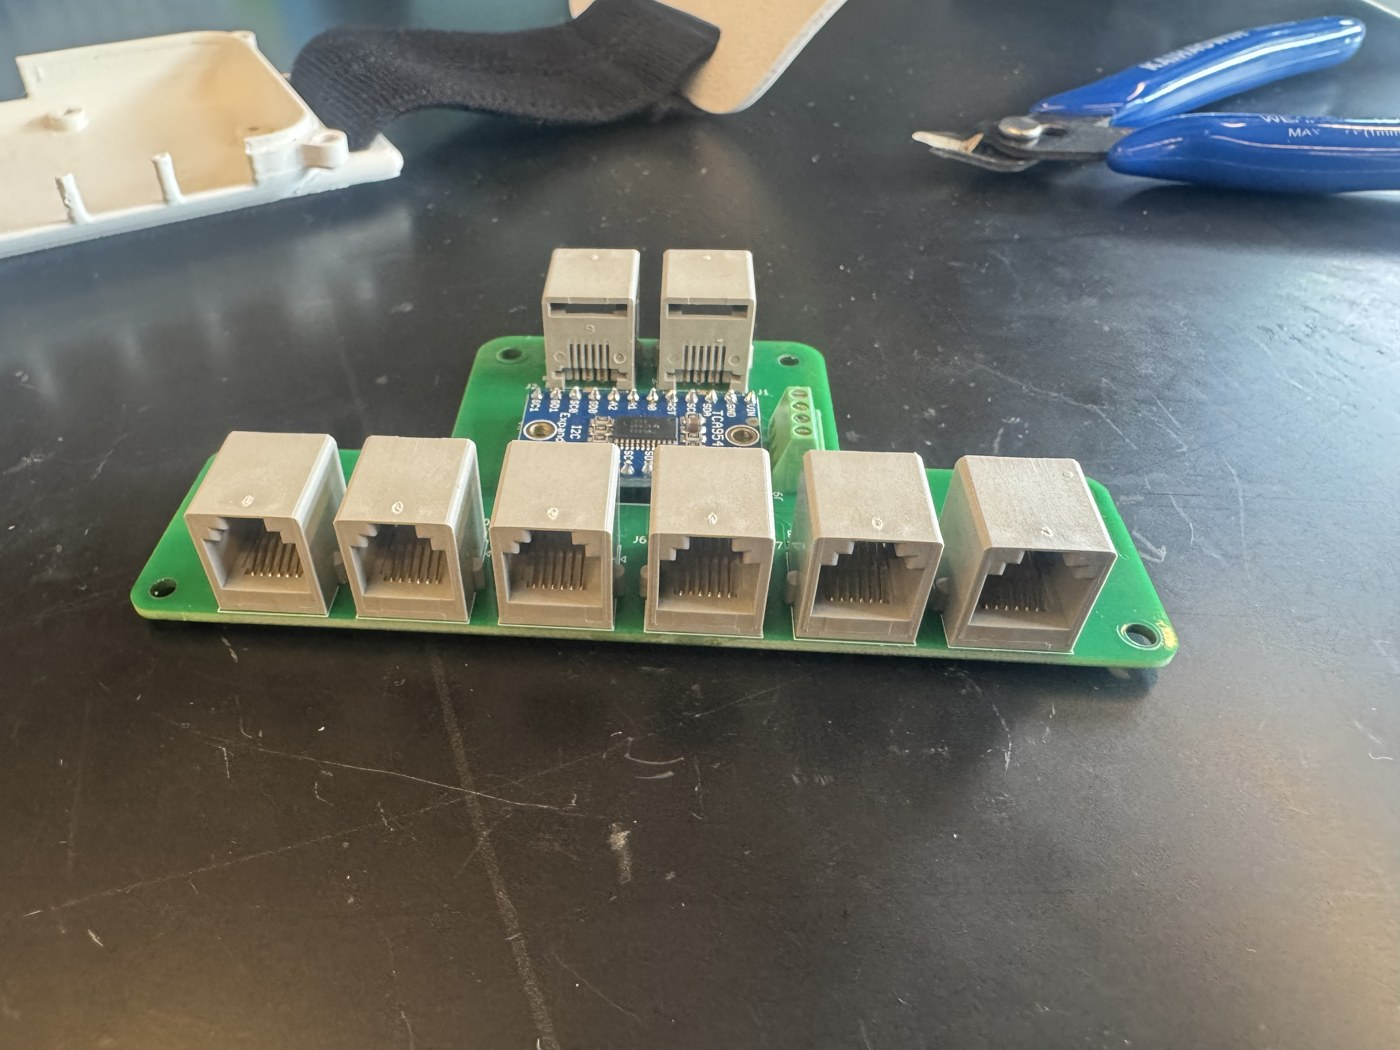
\includegraphics[width=\linewidth]{images/v1_pcb.jpg}
\end{minipage}\hfill
\begin{minipage}[t]{0.24\textwidth}
  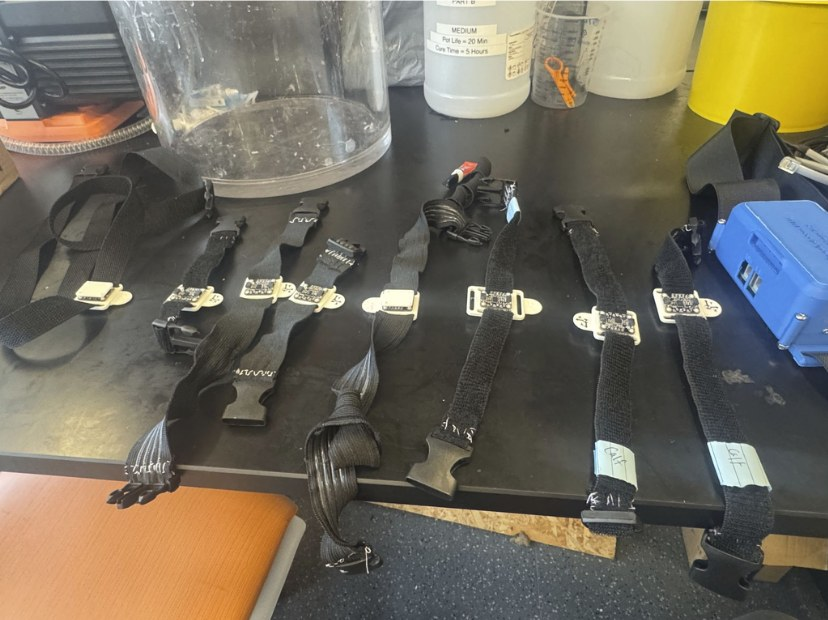
\includegraphics[width=\linewidth]{images/v1_nodes.jpg}
\end{minipage}\hfill
\begin{minipage}[t]{0.135\textwidth}
  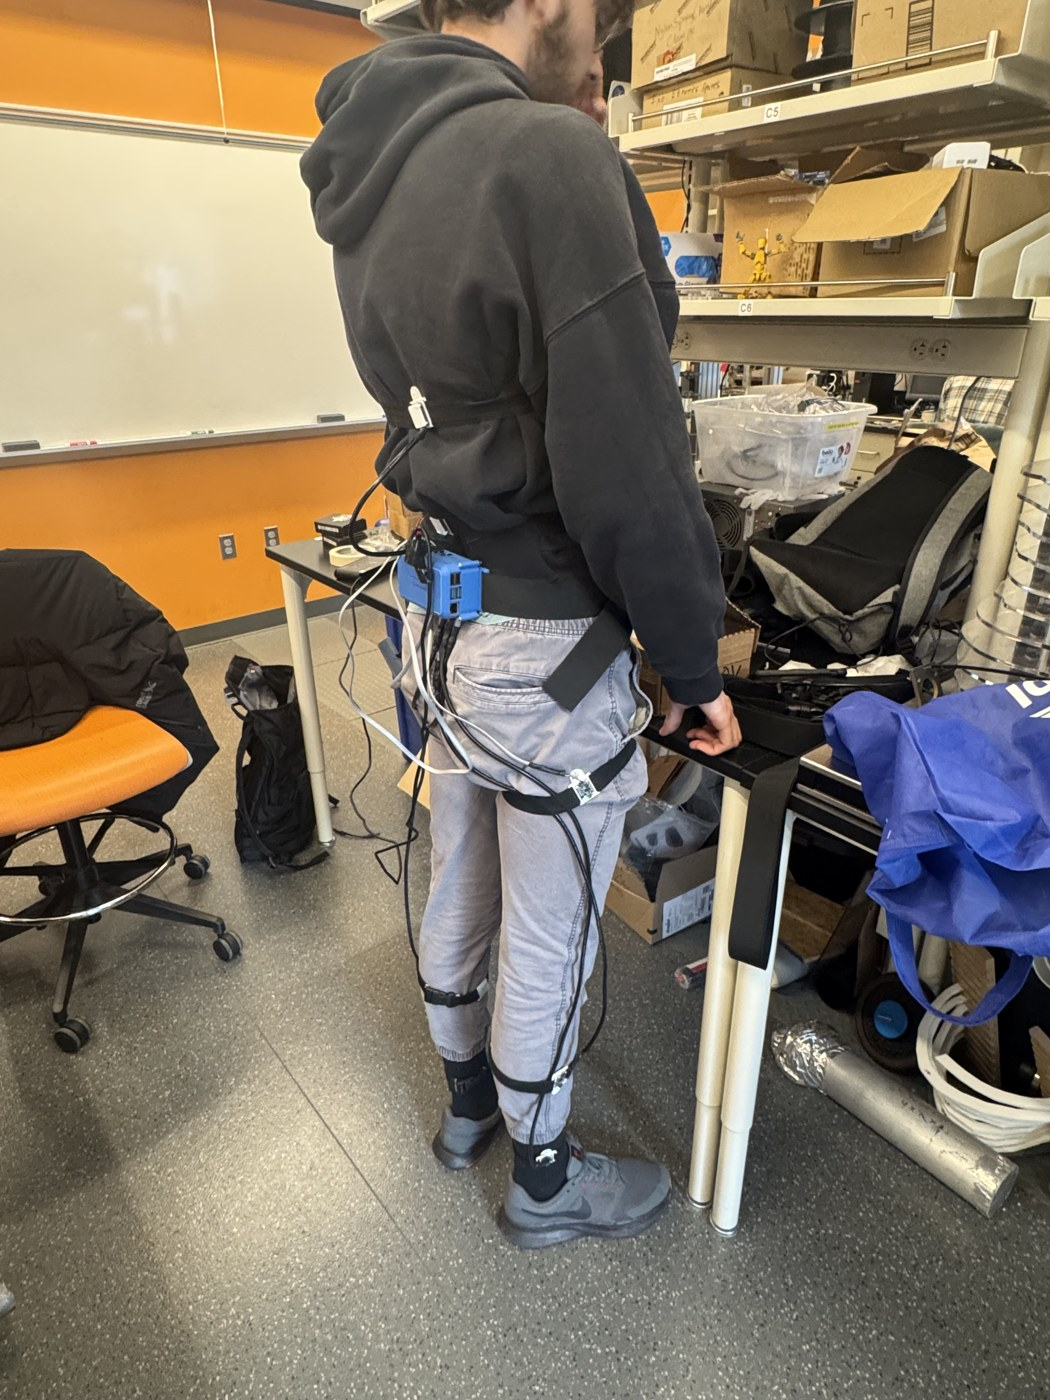
\includegraphics[width=\linewidth]{images/v1_worn_corner.jpg}
\end{minipage}\hfill
\begin{minipage}[t]{0.135\textwidth}
  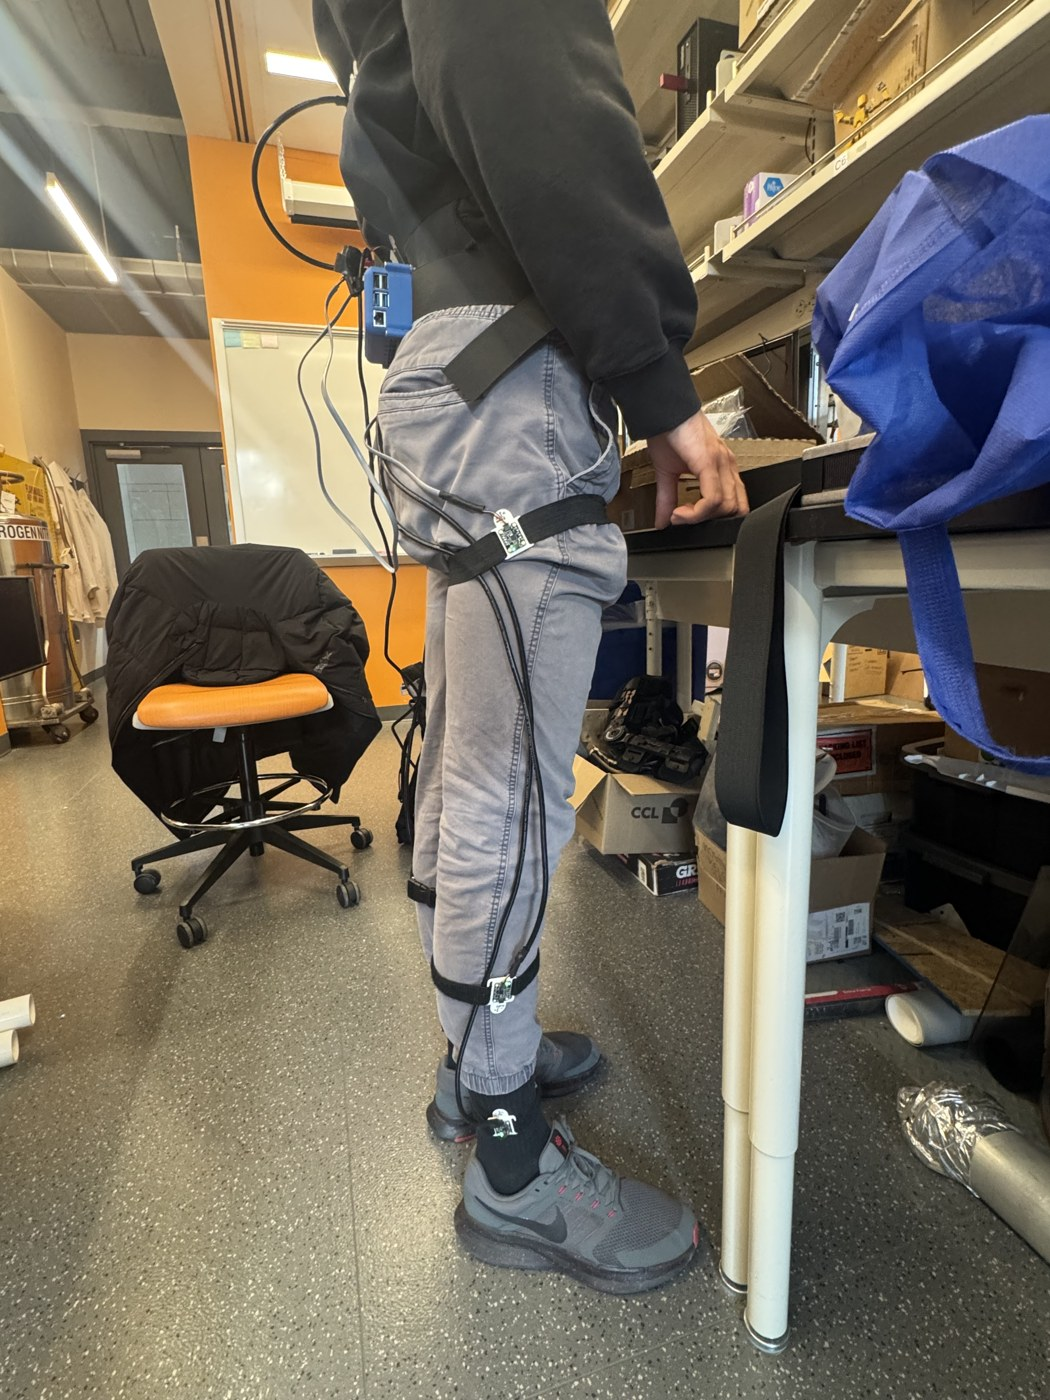
\includegraphics[width=\linewidth]{images/v1_worn_side.jpg}
\end{minipage}\hfill
\begin{minipage}[t]{0.24\textwidth}
  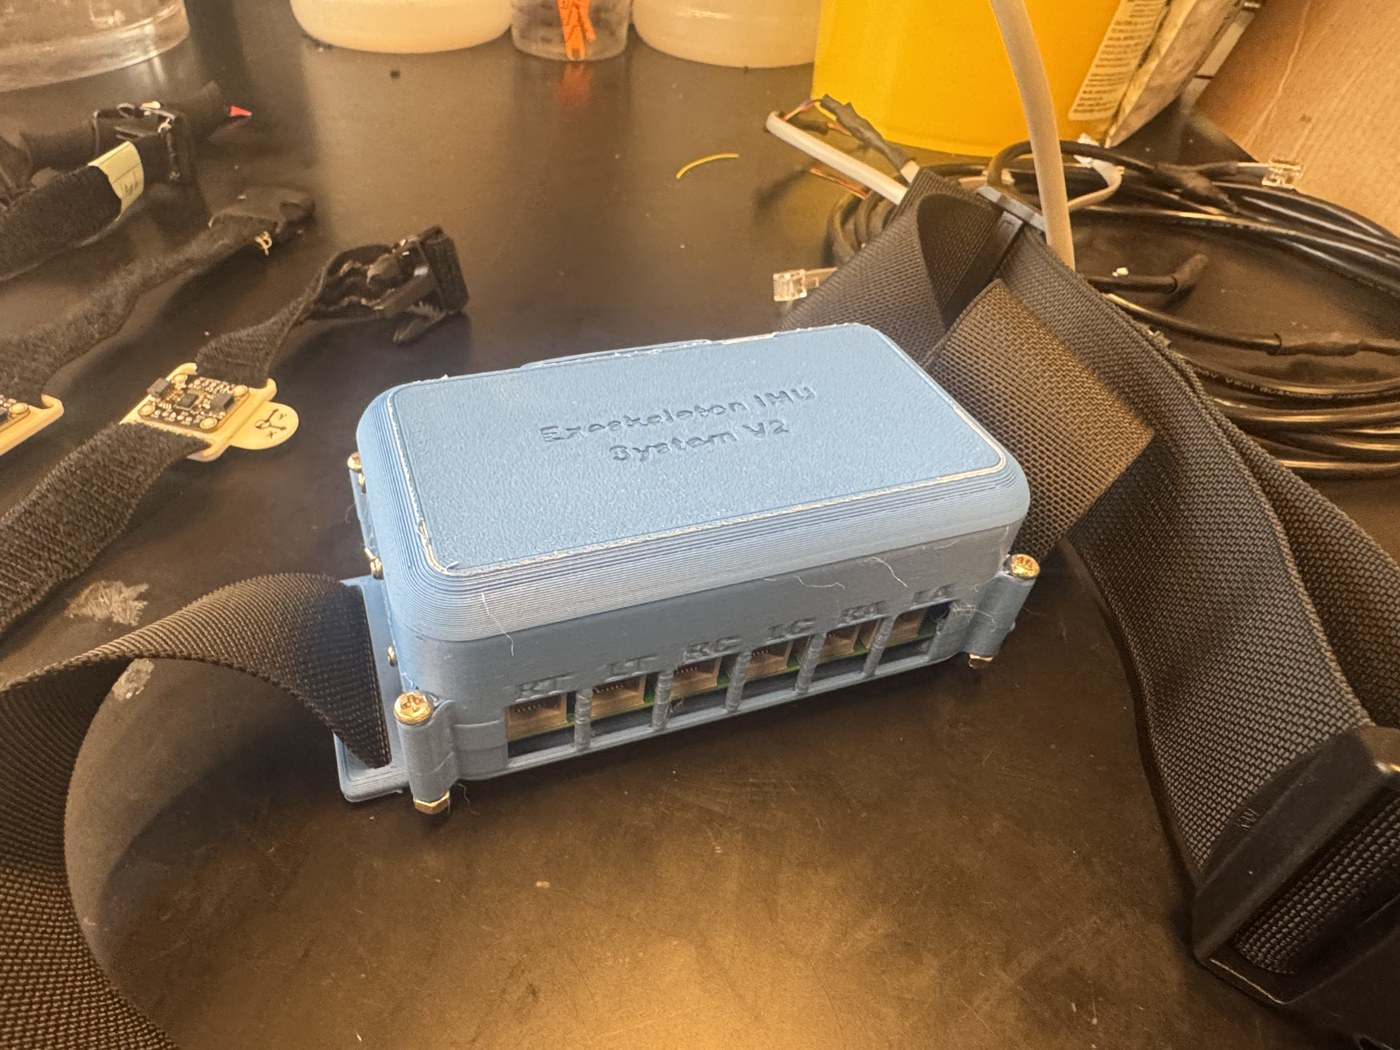
\includegraphics[width=\linewidth]{images/v1_hub.jpg}
\end{minipage}
\captiontext{IMU System V1, the original I\textsuperscript{2}C
architecture: fully assembled custom multiplexer PCB, the eight
body-segment sensor nodes on their straps, worn testing of the
first-generation array, and the belt-mounted acquisition hub with
per-segment channels.}

The Teensy 4.1 owns all sensor communication and streams normalized
quaternion data over serial to a Raspberry Pi running the gait-detection
algorithm; when the algorithm flags abnormal gait indicative of a potential
fall, it issues a serial command to a dedicated control board that actuates
the pneumatic cylinders to assist the user. This separation of concerns
dedicates the Pi to gait analysis, leaves headroom for algorithm growth,
and isolates data acquisition from processing. A 10-minute sustained trial
logging all eight IMUs simultaneously validated the system:

\begin{center}\small
\begin{tabular}{@{}ll@{}}
\toprule
\textbf{Metric} & \textbf{Result} \\
\midrule
Sampling rate          & 400\,Hz sustained (ref.: Delsys 120\,Hz, Xsens 240\,Hz) \\
Packet interval        & $<$2.5\,ms consistent \\
Packet loss            & 0.0\% \\
Mean orientation error & 0.003\% (unit-quaternion magnitude deviation) \\
\bottomrule
\end{tabular}
\end{center}

\vspace{4pt}
\begin{minipage}[t]{0.305\textwidth}
  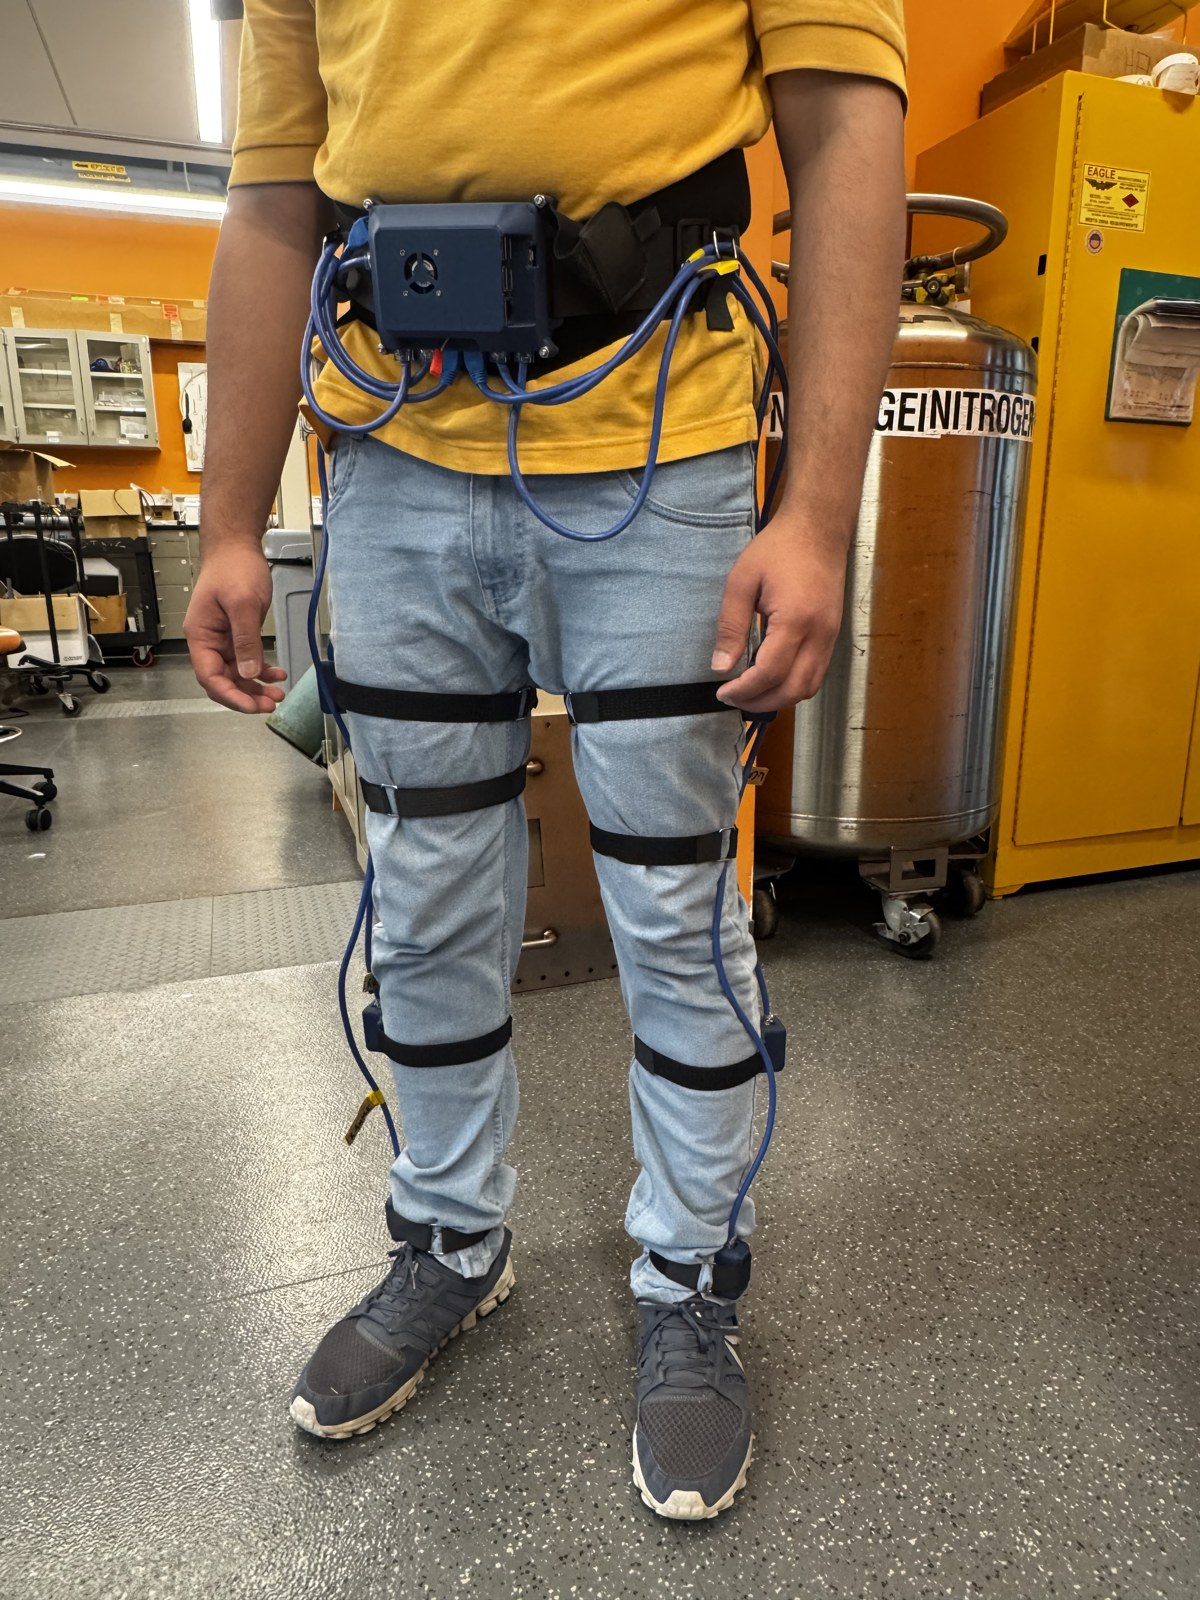
\includegraphics[width=\linewidth]{images/worn_system.jpg}
  \captiontext{IMU System V2 worn for data acquisition: each sensor at
  its designated anatomical location on custom adjustable straps.}
\end{minipage}\hfill
\begin{minipage}[t]{0.305\textwidth}
  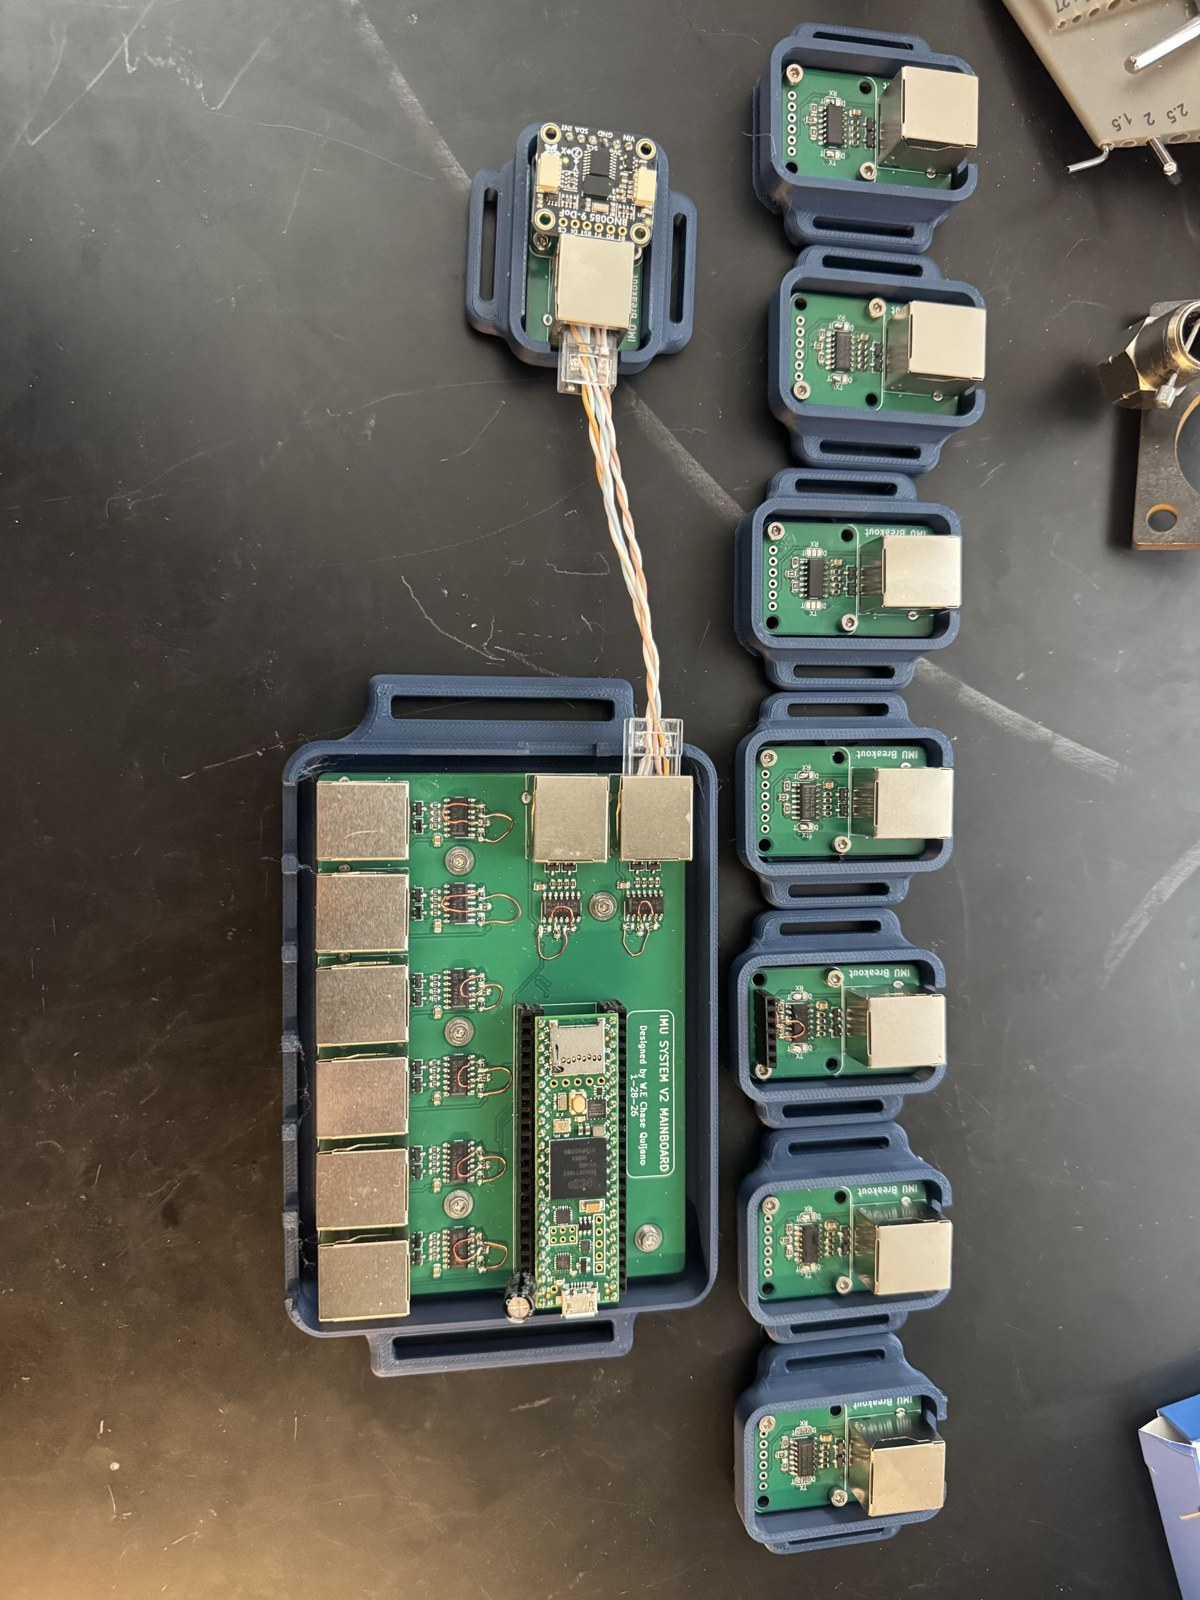
\includegraphics[width=\linewidth]{images/mainboard_nodes.jpg}
  \captiontext{Custom Teensy 4.1 mainboard and BNO085 sensor nodes:
  simultaneous logging at up to 400\,Hz per node over the full-duplex
  RS-485 matrix.}
\end{minipage}\hfill
\begin{minipage}[t]{0.34\textwidth}
  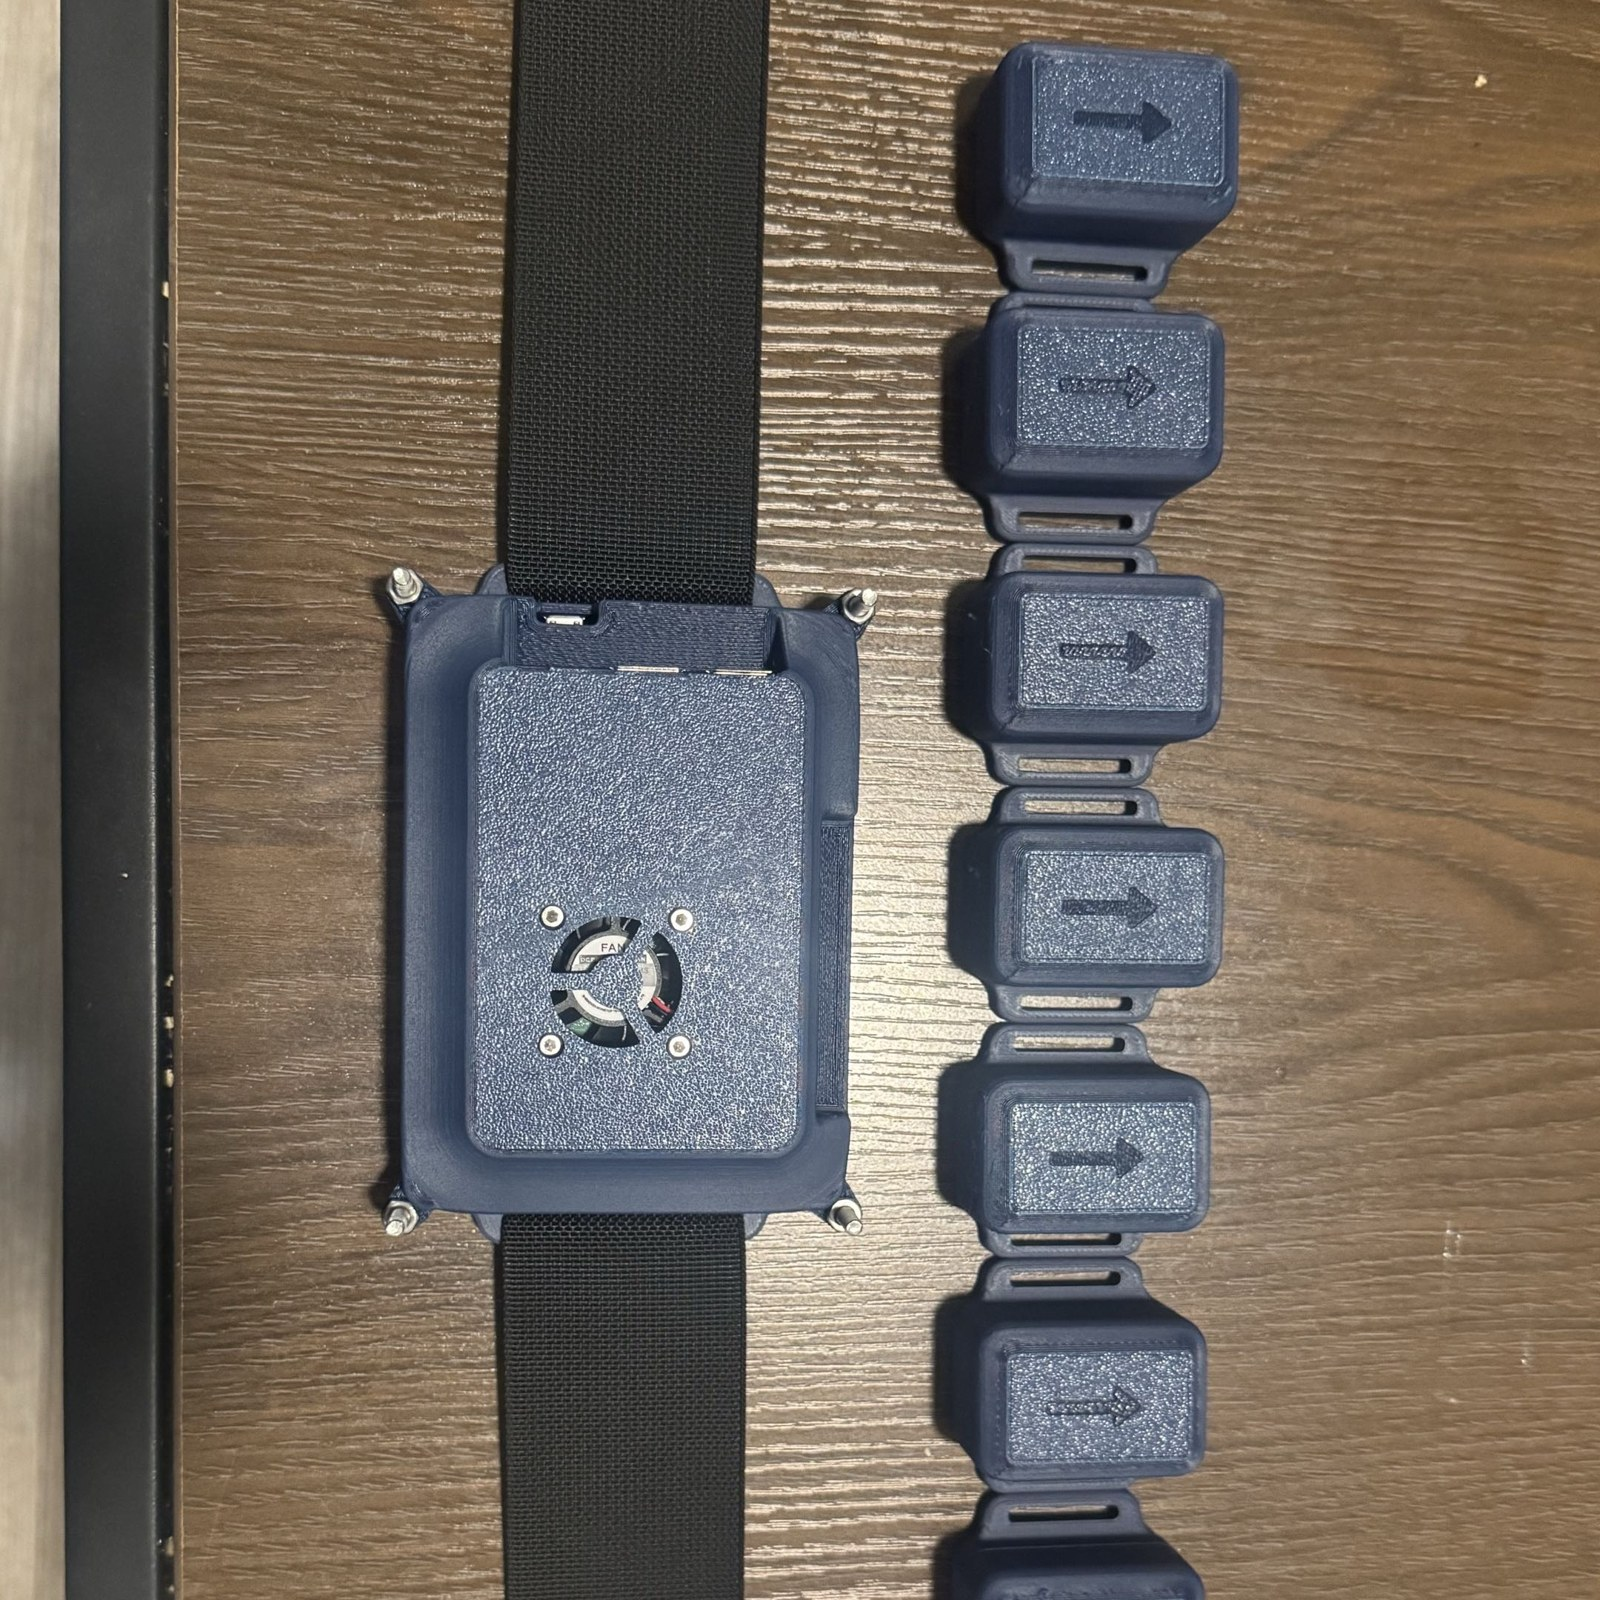
\includegraphics[width=\linewidth]{images/enclosures.jpg}
  \captiontext{Assembled 8-node array: compact, low-profile modular
  housings keep hardware light, secure, and unobtrusive during human
  movement testing.}
\end{minipage}

\vspace{4pt}
\begin{minipage}[t]{0.475\textwidth}
  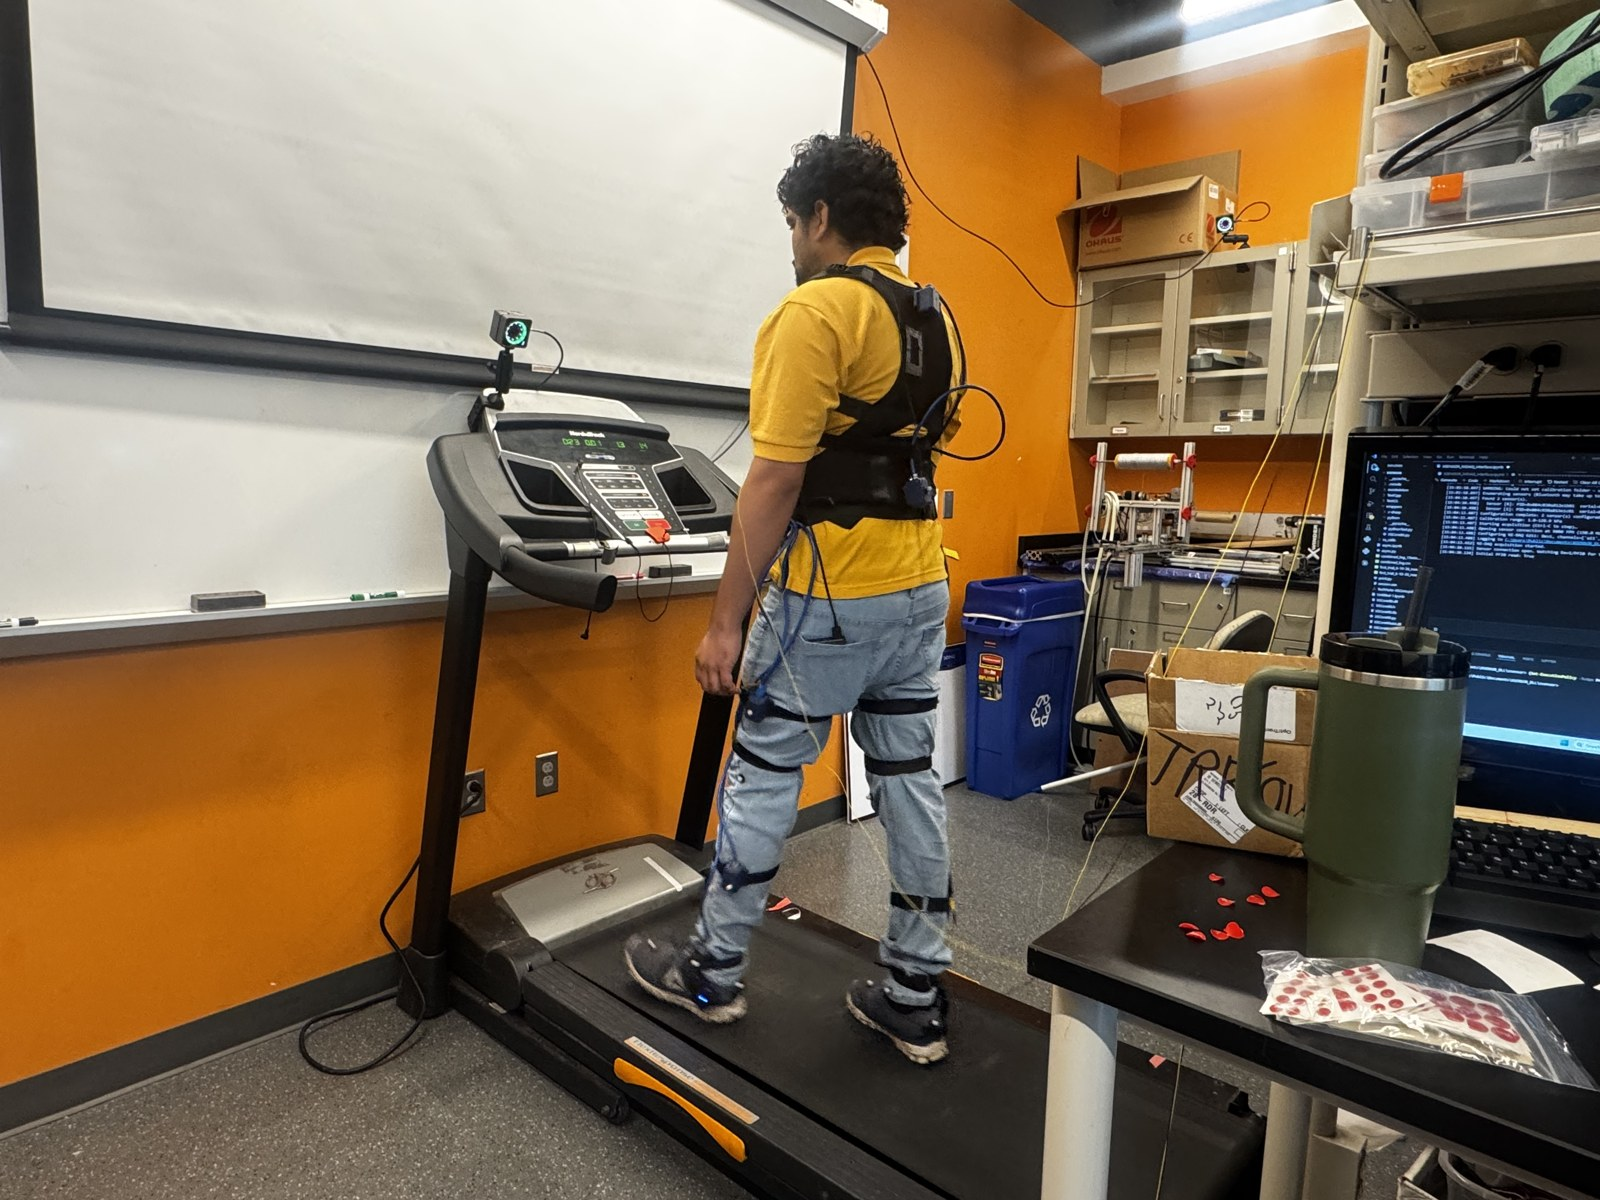
\includegraphics[width=\linewidth]{images/treadmill.jpg}
  \captiontext{Treadmill walking trial with the IMU system worn,
  validated simultaneously against an OptiTrack optical motion-capture
  system, with reflective markers tracked alongside the IMU array.}
\end{minipage}\hfill
\begin{minipage}[t]{0.475\textwidth}
  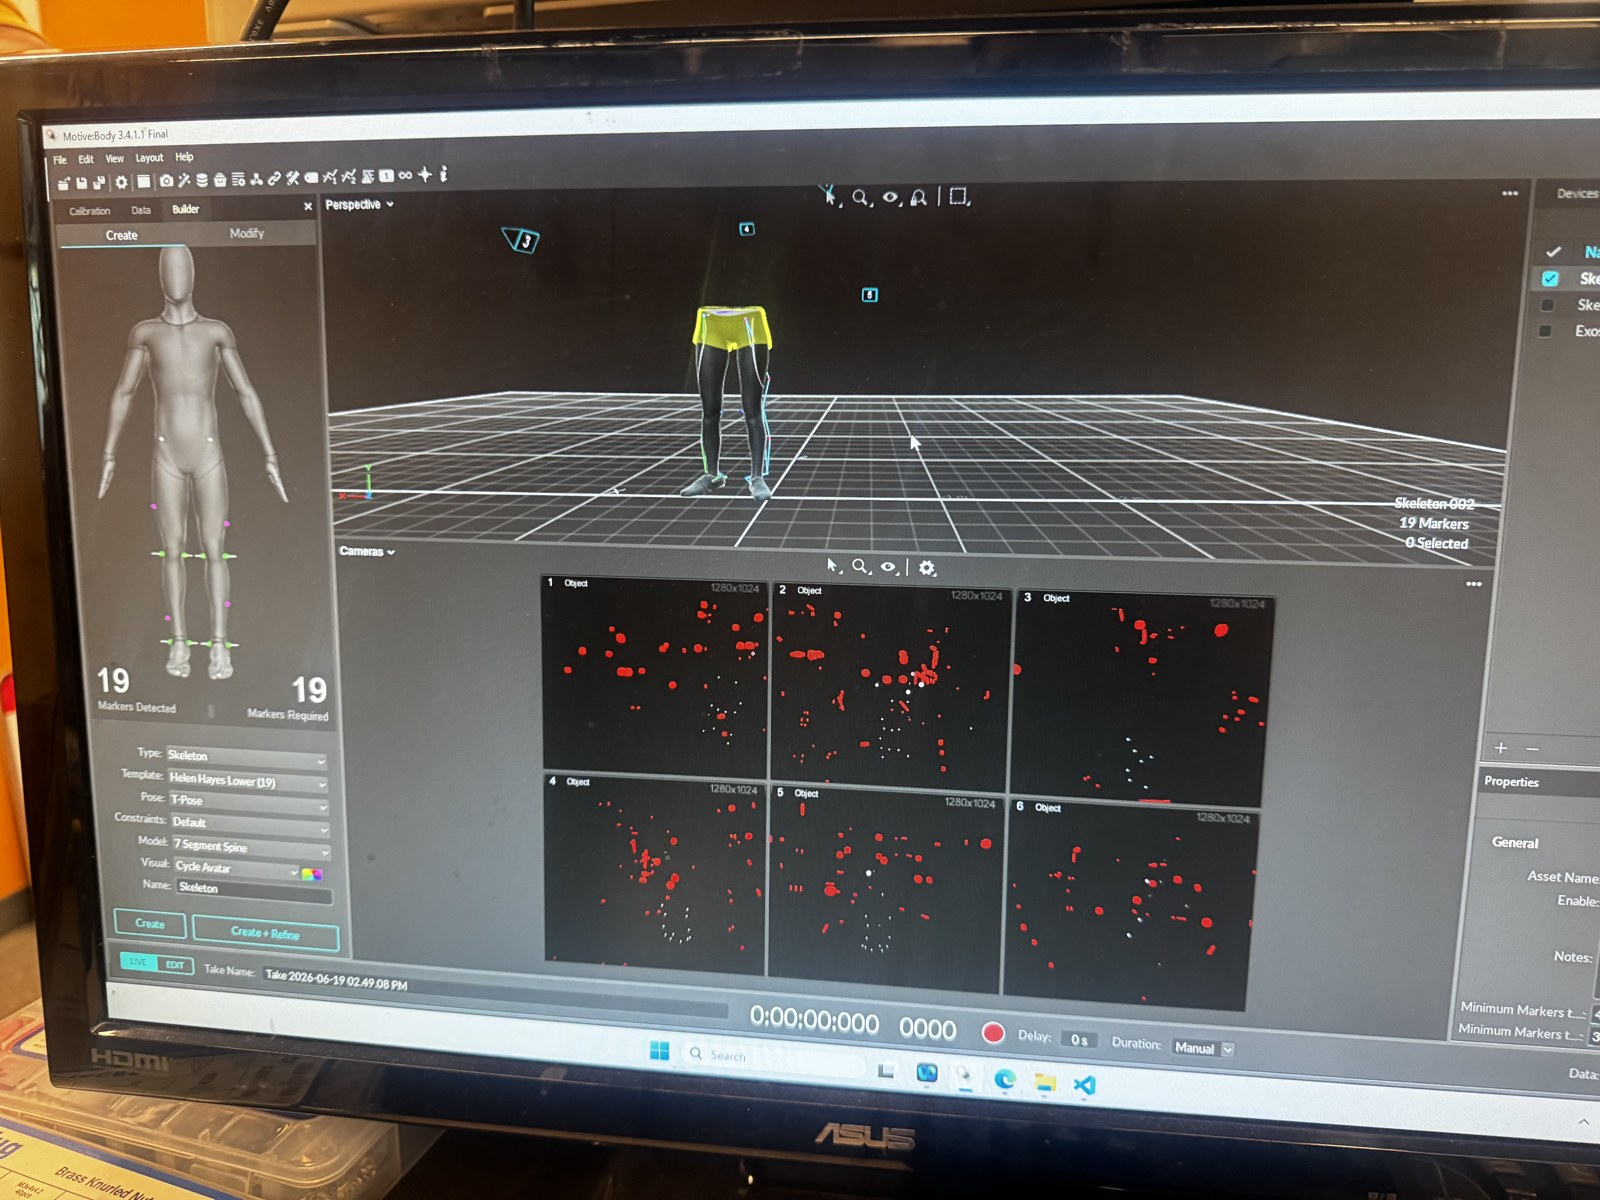
\includegraphics[width=\linewidth]{images/optitrack.jpg}
  \captiontext{OptiTrack Motive software reconstructing the
  reflective-marker skeleton in real time during the walking trials,
  serving as optical ground truth alongside the IMU data.}
\end{minipage}

\subsection*{Test Bench V2}

The original plywood test bench proved the concept but had an impractical
footprint, and its 3D-printed cylinder mounts lacked the rigidity required
for reliable actuation under pneumatic load. The revised bench is built on
a laser-cut wood chassis that significantly reduces the footprint while
improving structural rigidity, and adds the functional features testing
actually needed:

\begin{itemize}
  \item Emergency-stop button for immediate system shutoff during testing.
  \item Dedicated toggle switches for the 15\,V and 5\,V power rails for
        manual line-level control during debugging and evaluation.
  \item A single centralized pneumatic line feeding all solenoids,
        for simplified routing and fast pressurization between test cycles.
  \item An integrated pressure transducer for real-time pressure readings
        during data acquisition, and improved cable management to reduce
        wiring clutter and accidental disconnections.
\end{itemize}

\vspace{2pt}
\begin{minipage}[t]{0.53\textwidth}
  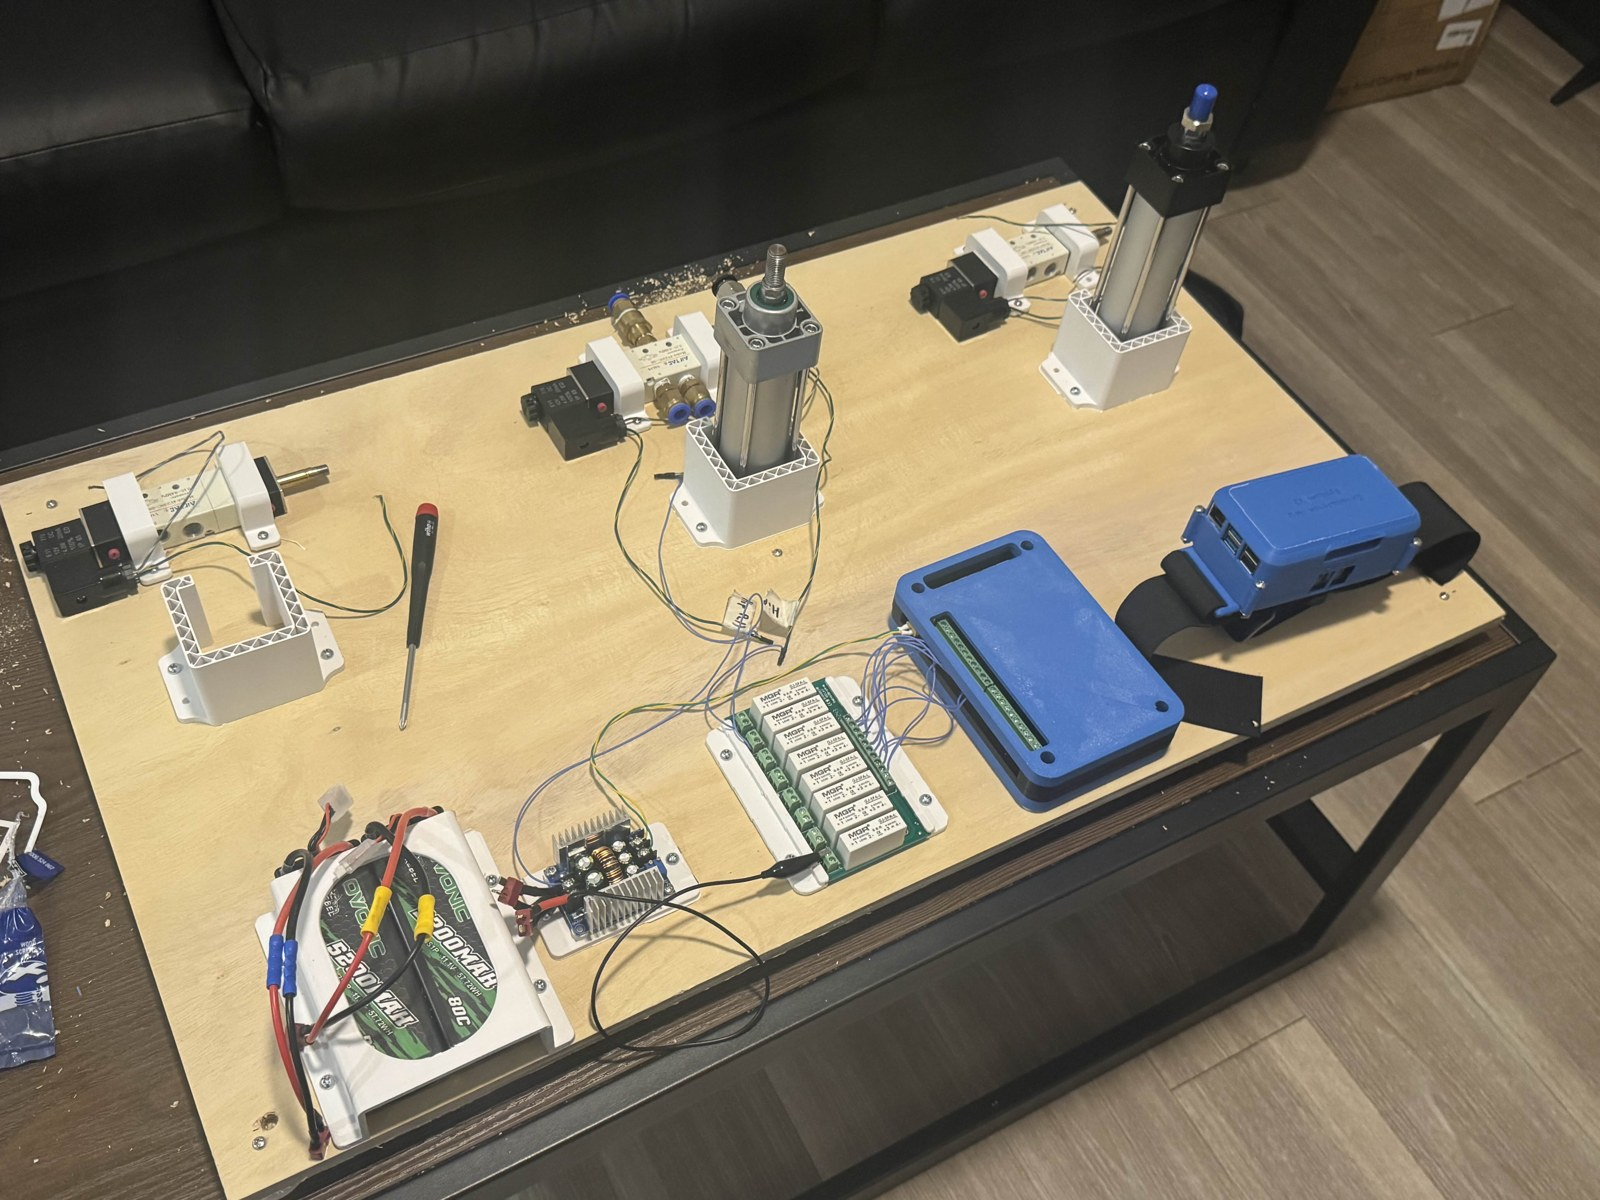
\includegraphics[width=\linewidth]{images/testbench_v1.jpg}
  \captiontext{Original plywood test bench: 3D-printed component
  mounts, series LiPo power, and the first pneumatic cylinder and
  solenoid layout.}
\end{minipage}\hfill
\begin{minipage}[t]{0.40\textwidth}
  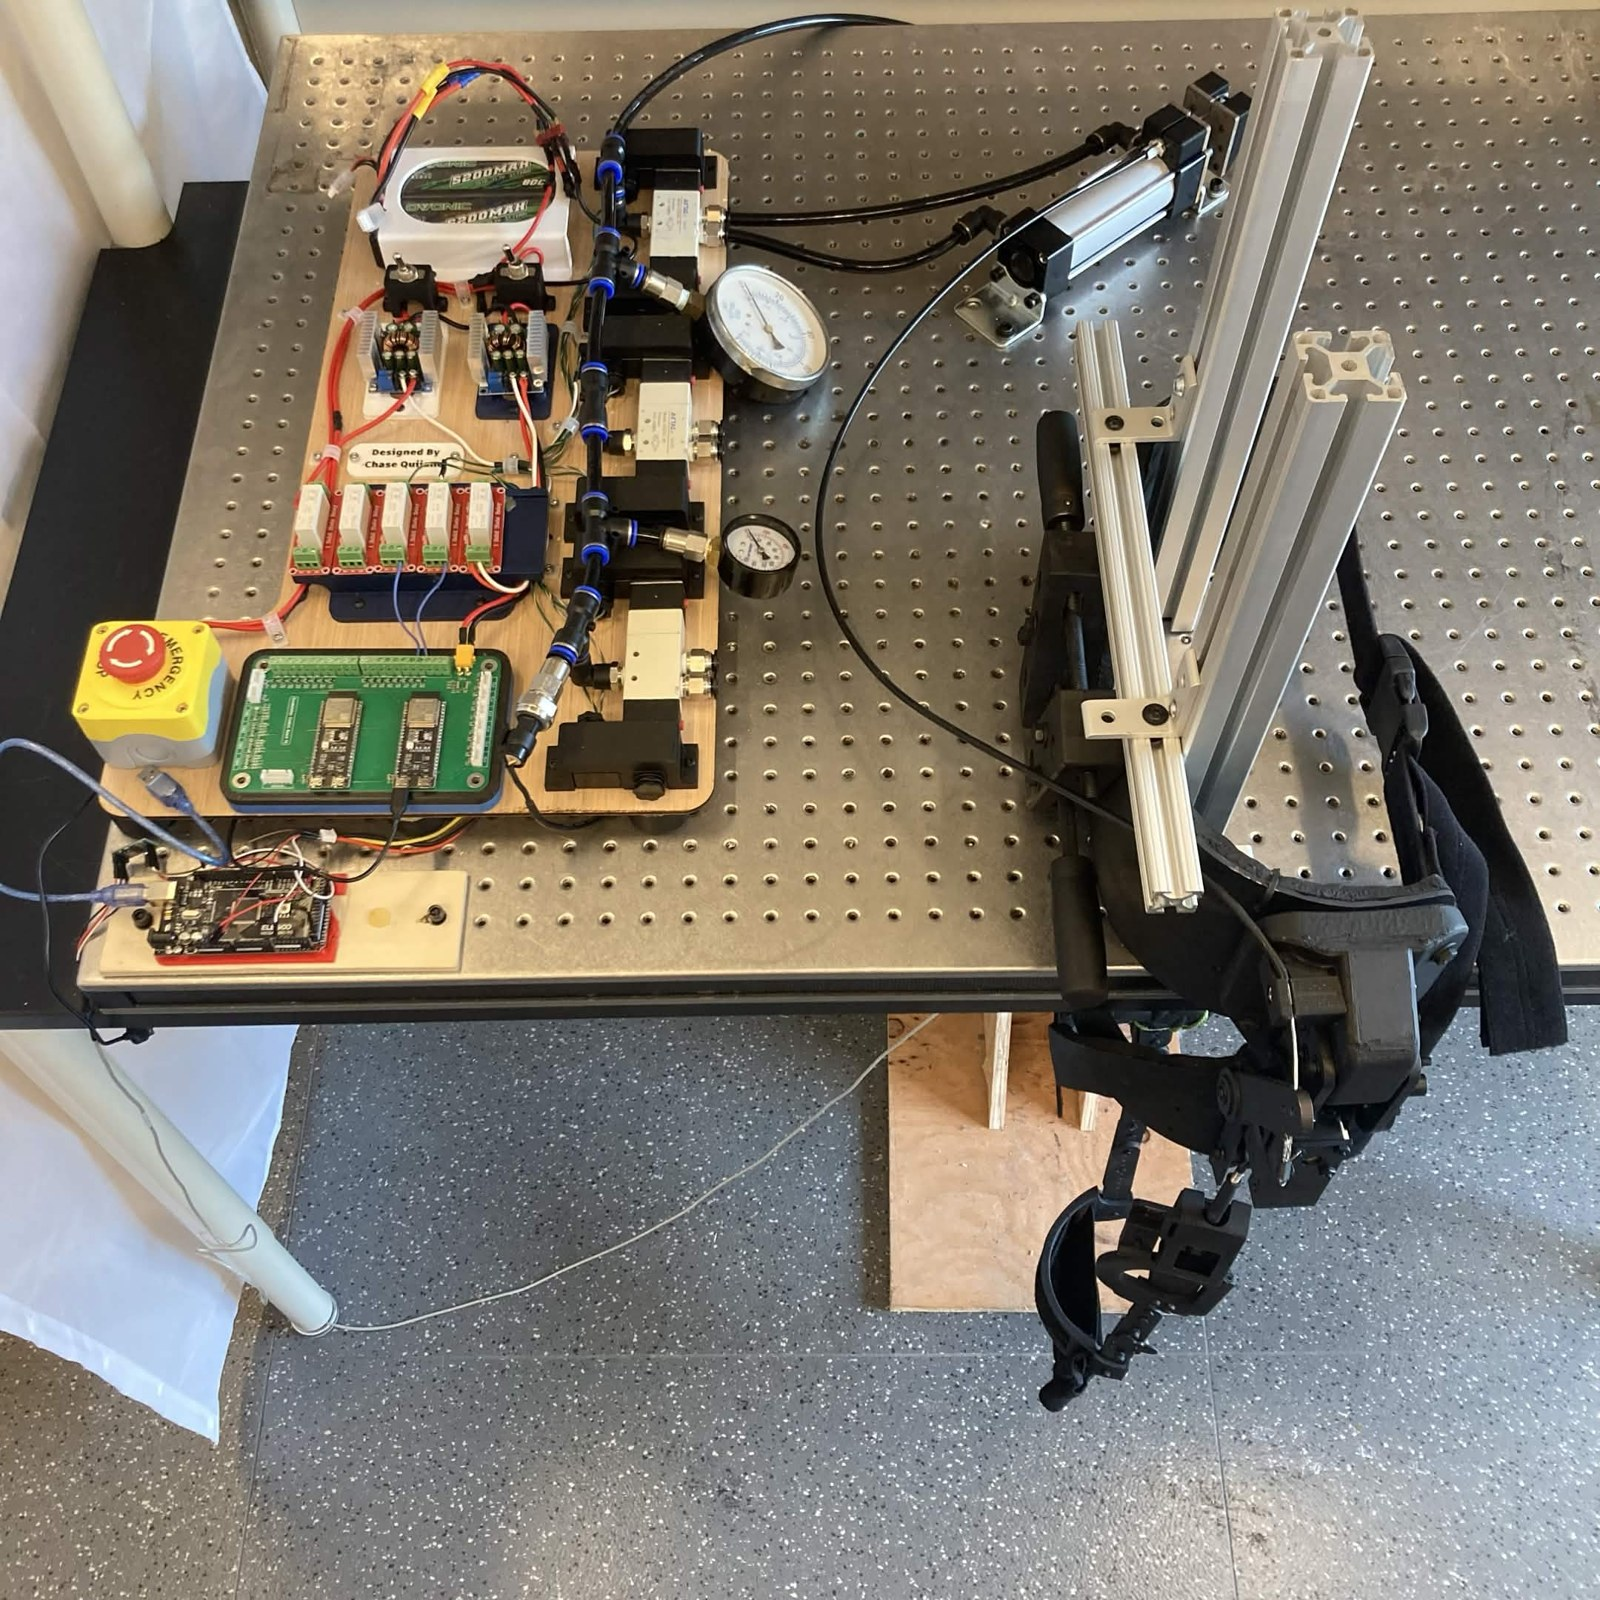
\includegraphics[width=\linewidth]{images/testbench_actual.jpg}
  \captiontext{Test Bench V2 laid out and prepared for hip-abduction
  load-cell data acquisition: E-stop, switched power rails, centralized
  pneumatic line, and integrated pressure transduction.}
\end{minipage}

\subsection*{Hip Abduction Load-Cell Testing}

Characterizing the exoskeleton's force output was a primary objective. The
chassis was fixed to a threaded steel table with a horizontal load-cell
fixture mounted parallel to the exoskeleton leg, connected by a rope under
tension with the static tension accounted for in all readings. A linear
calibration model was derived from the manufacturer's documentation and
verified through static trials. A standardized procedure governed every
run: regulator setpoint, actuation delay configured in the control-board
DAQ firmware, and a MATLAB DAQ script with output files named by trial
number, pressure, and delay for traceability.

A total of 96 trials were completed across a matrix of four actuation
delays (40, 50, 60, 80\,ms) and six supply pressures (50--100\,PSI). The
collected data has been validated as viable, with trend analysis across
the parameter space ongoing.

\vspace{2pt}
\begin{minipage}[t]{0.70\textwidth}
  
\includegraphics[width=\linewidth]{images/torque_plot.jpg}
  \captiontext{Hip abduction load-cell results: supply pressure (PSI)
  against applied torque (N$\cdot$m) across the 96-trial matrix.}
\end{minipage}\hfill
\begin{minipage}[t]{0.26\textwidth}
  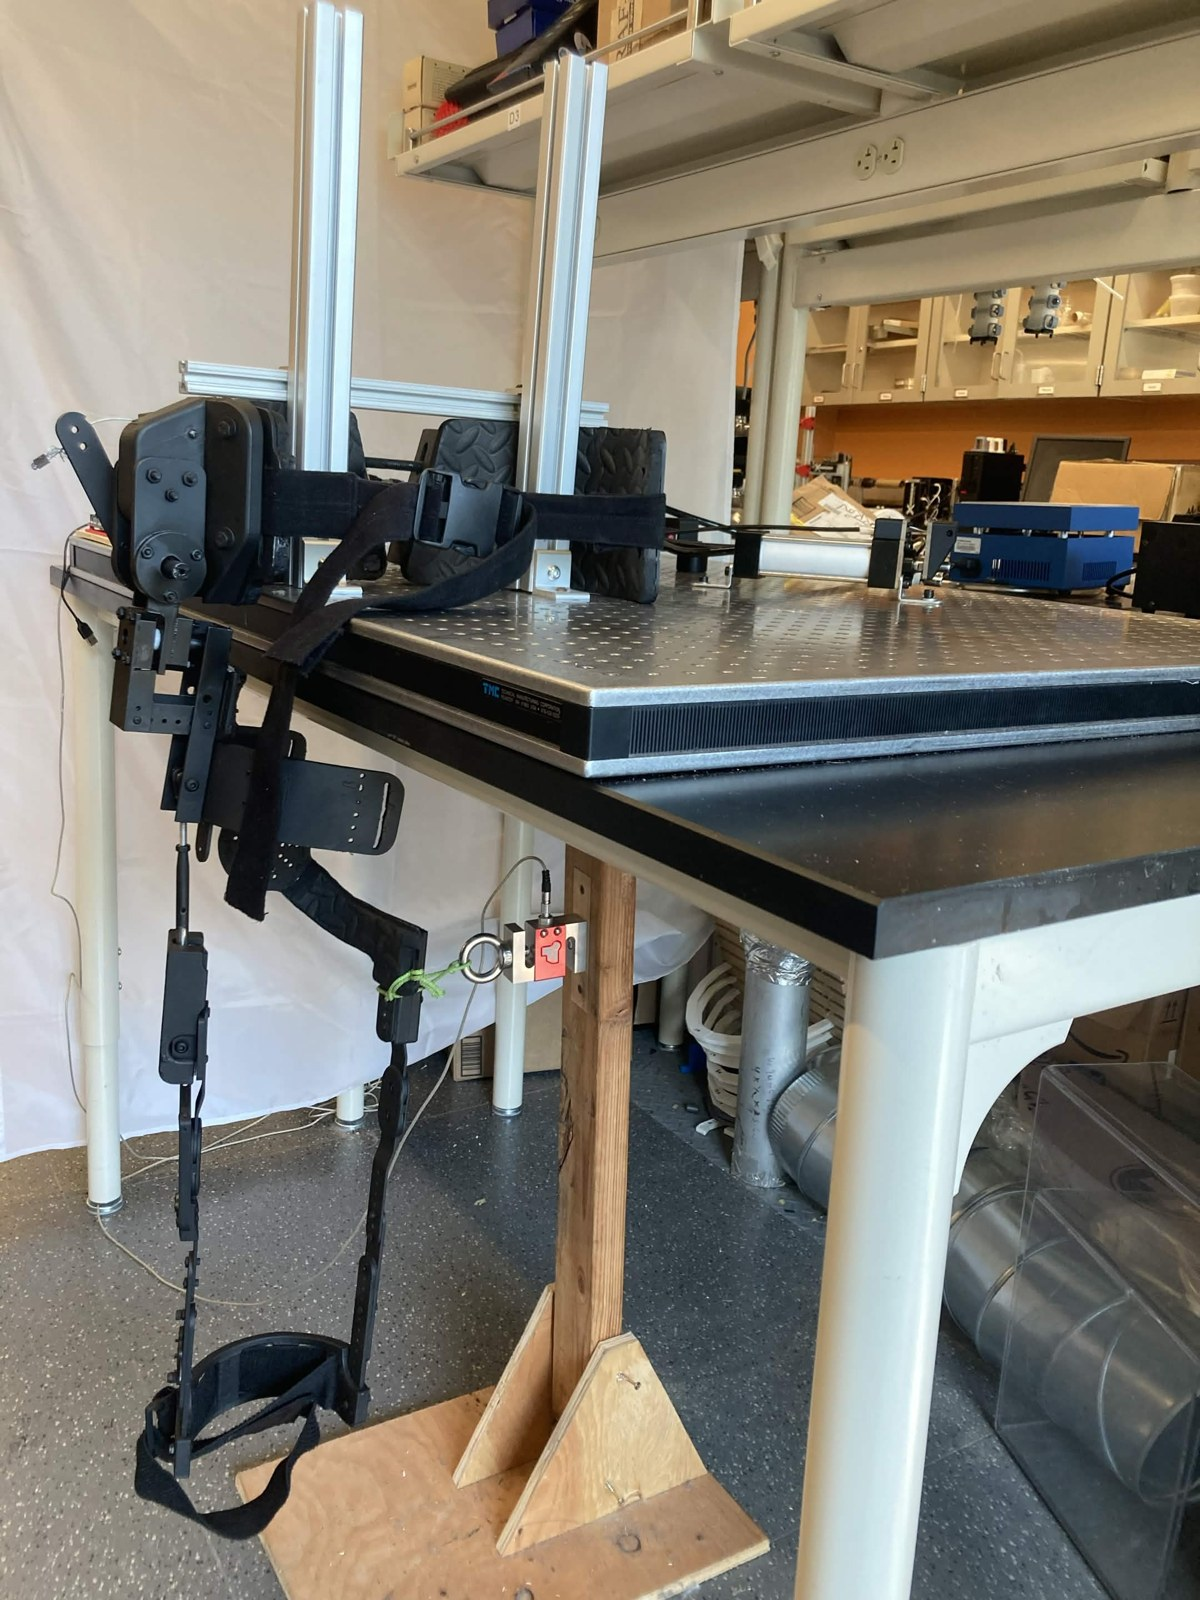
\includegraphics[width=\linewidth]{images/force_stand.jpg}
  \captiontext{Hip mechanism on the force-testing stand with the load cell
  inline, the fixture behind the trial campaigns.}
\end{minipage}

\subsection*{Modular Pneumatic Cylinder Assembly}

Fixed, crimped Bowden-cable fittings on the pneumatic cylinders made
modifications and component swaps time-consuming in earlier iterations. I
addressed this with a modular cable-retention mechanism developed by
reverse-engineering a bicycle brake-lever assembly: a keyed steel piece on
a swiveling axis locks the cable end-bead in place, allowing tool-free
cable removal. The first-generation assembly was constructed from
1/4$''$ waterjet-cut steel and ABS to maintain structural integrity under
cyclic loading.

\vspace{2pt}
\begin{center}
\begin{minipage}[t]{0.55\textwidth}
  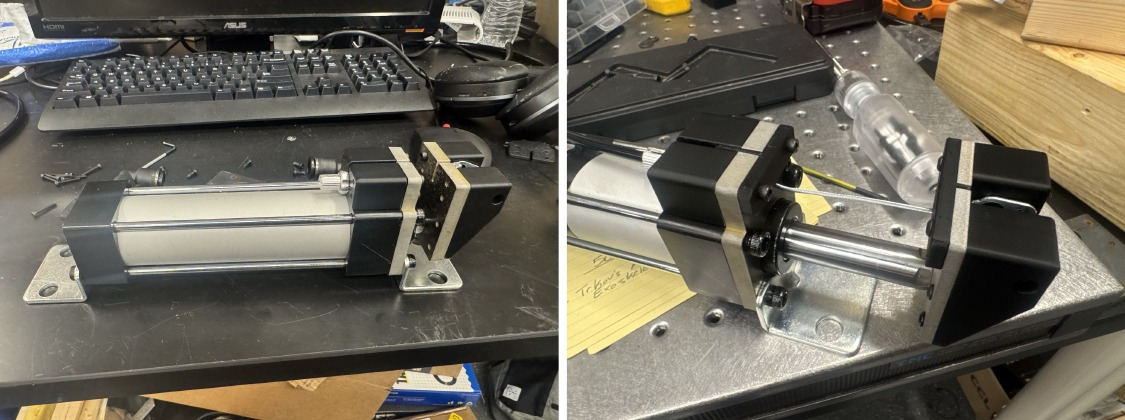
\includegraphics[width=\linewidth]{images/cylinder_assembly.jpg}
  \captiontext{First-generation modular pneumatic cylinder assembly:
  tool-free Bowden-cable retention adapted from a bicycle brake-lever
  mechanism.}
\end{minipage}
\end{center}

The second-generation mechanism adds a custom mount for a string
potentiometer, enabling closed-loop position control in a compact form
factor, and replaces the waterjet-cut steel plates with waterjet-cut
aluminum for weight reduction ahead of its integration into the wearable
backpack.

\vspace{2pt}
\begin{minipage}[t]{0.50\textwidth}
  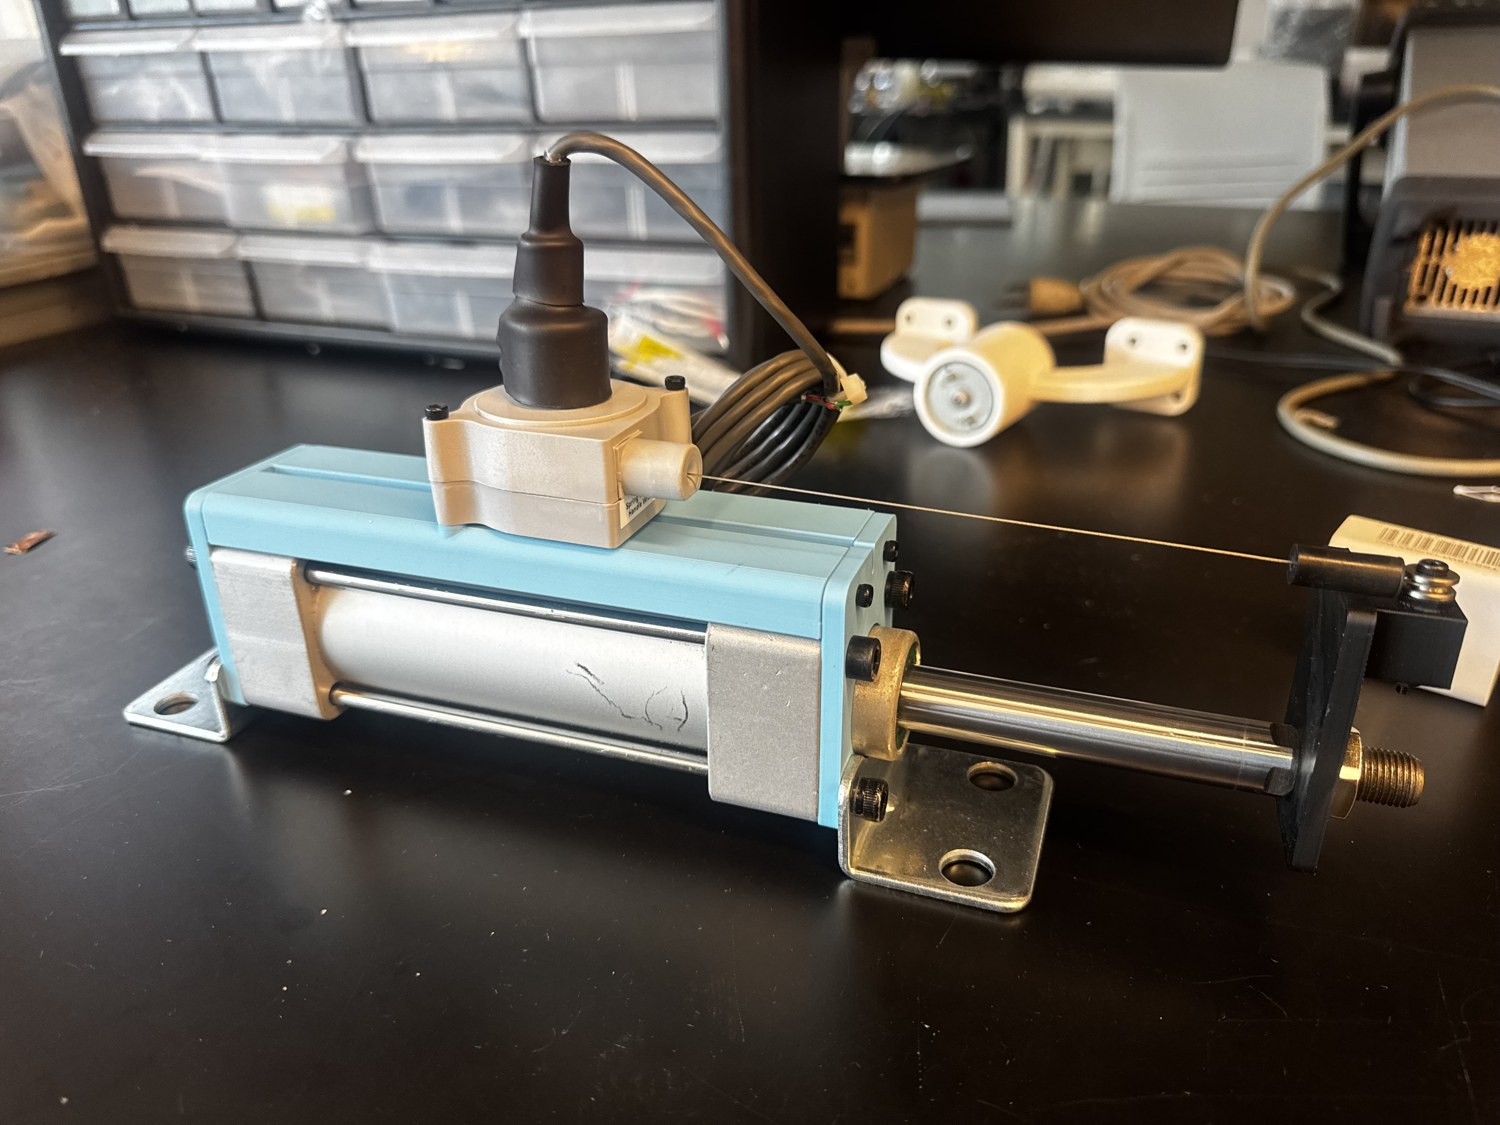
\includegraphics[width=\linewidth]{images/v2_cyl_side.jpg}
  \captiontext{Cylinder mechanism V2: string potentiometer on its
  custom mount with the wire routed to the rod end for closed-loop
  position feedback.}
\end{minipage}\hfill
\begin{minipage}[t]{0.28\textwidth}
  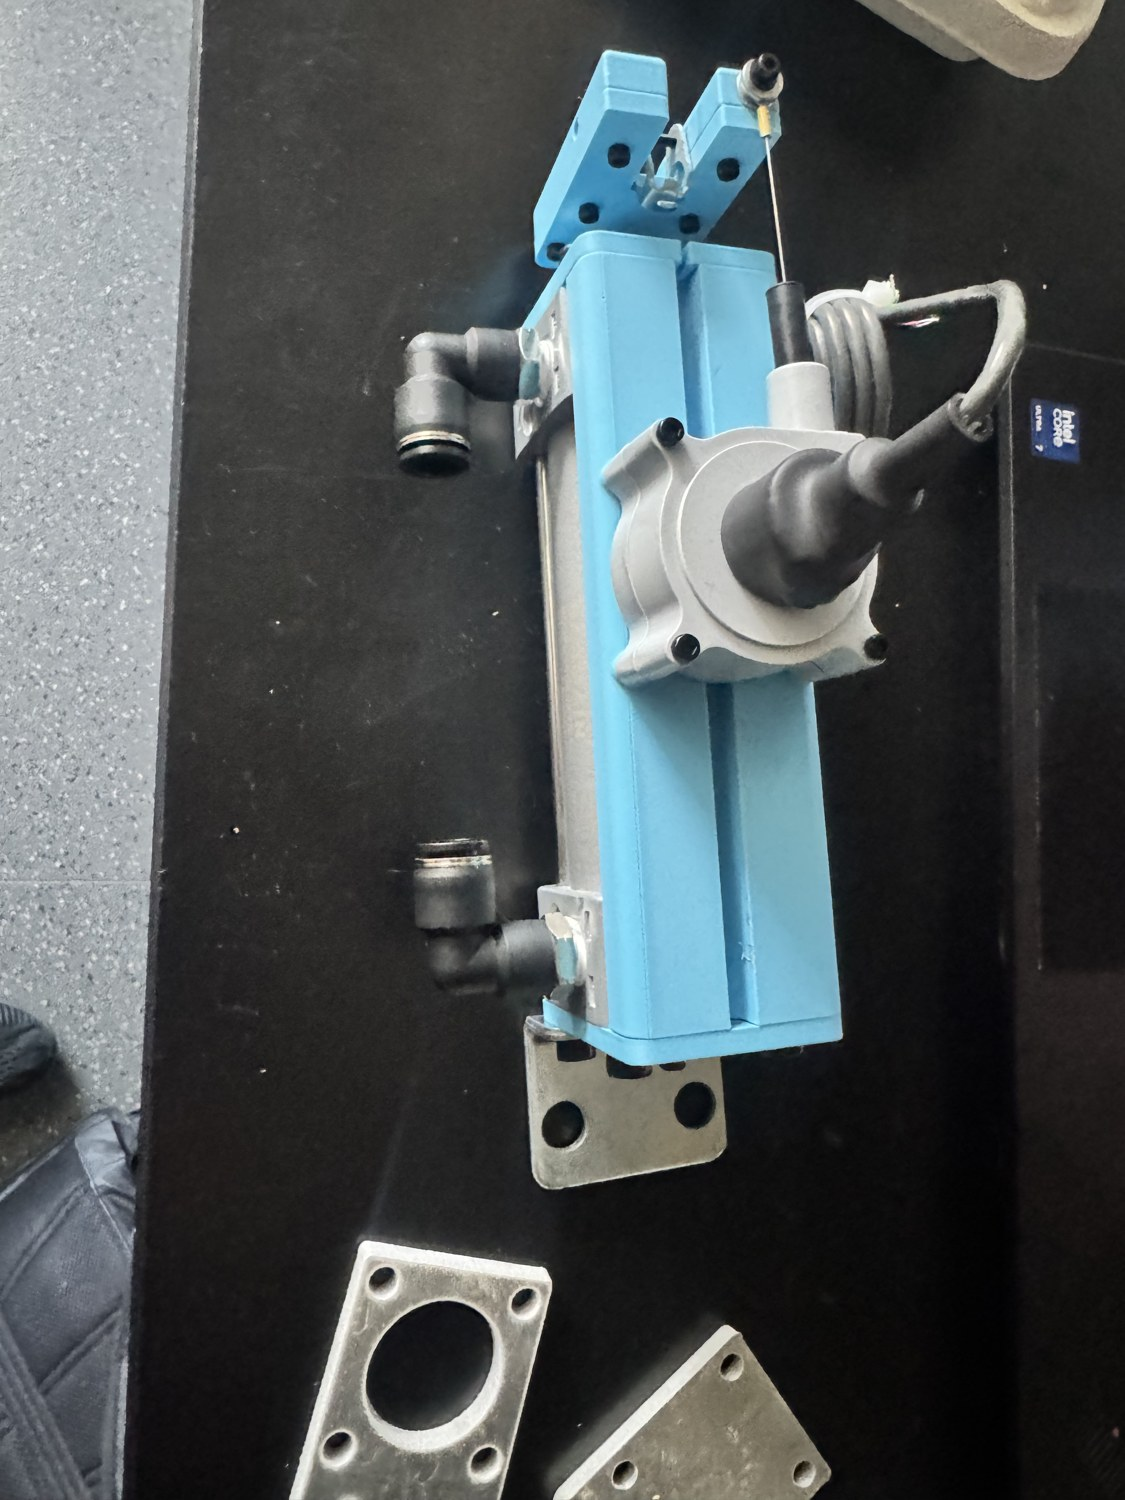
\includegraphics[width=\linewidth]{images/v2_cyl_mount.jpg}
  \captiontext{V2 assembly with waterjet-cut aluminum mounting plates,
  replacing the previous steel for weight reduction.}
\end{minipage}

\vspace{3pt}
{\footnotesize\sloppy
\textbf{Published work from this research program.} The exoskeleton
program builds on the following publications by our group:
\begin{enumerate}[leftmargin=1.5em,itemsep=1pt,topsep=2pt]
  \item V. Varma, S. N. Patel, N. P. Wilson, and M. Trkov,
        ``Characterization of Hip Abduction Exoskeleton for Assistance
        During Gait Perturbations,'' \textit{IEEE/ASME International
        Conference on Advanced Intelligent Mechatronics (AIM)}, 2024.
        doi:10.1109/AIM55361.2024.10637061.
  \item V. Varma and M. Trkov, ``Intersegmental coordination in human
        slip perturbation responses,'' \textit{Journal of Biomechanics},
        vol.~168, art.~112097, 2024.
        doi:10.1016/j.jbiomech.2024.112097.
  \item V. Varma and M. Trkov, ``Investigation of intersegmental
        coordination patterns in human walking,'' \textit{Gait \&
        Posture}, vol.~112, pp.~88--94, 2024.
        doi:10.1016/j.gaitpost.2024.05.010.
  \item V. Varma, Z. Roberts, F. Mallick, and M. Trkov, ``Estimating
        Human-Exoskeleton Interaction Forces Using an Instrumented Thigh
        Brace and OpenSim,'' \textit{IFAC-PapersOnLine}, vol.~59,
        no.~30, pp.~353--358, 2025 (5th Conference on Modeling,
        Estimation and Control, MECC 2025).
        doi:10.1016/j.ifacol.2025.12.262.
\end{enumerate}}

\subsection*{Current Work \& Path to Human Trials}

Biomechanics testing is now underway, work I carry out alongside PhD
student Vaibhavsingh Varma: worn trials with the full system (harness,
exoskeleton, and IMU sensing network together) conducted on an overhead
safety tether.

\vspace{2pt}
\begin{minipage}[t]{0.20\textwidth}
  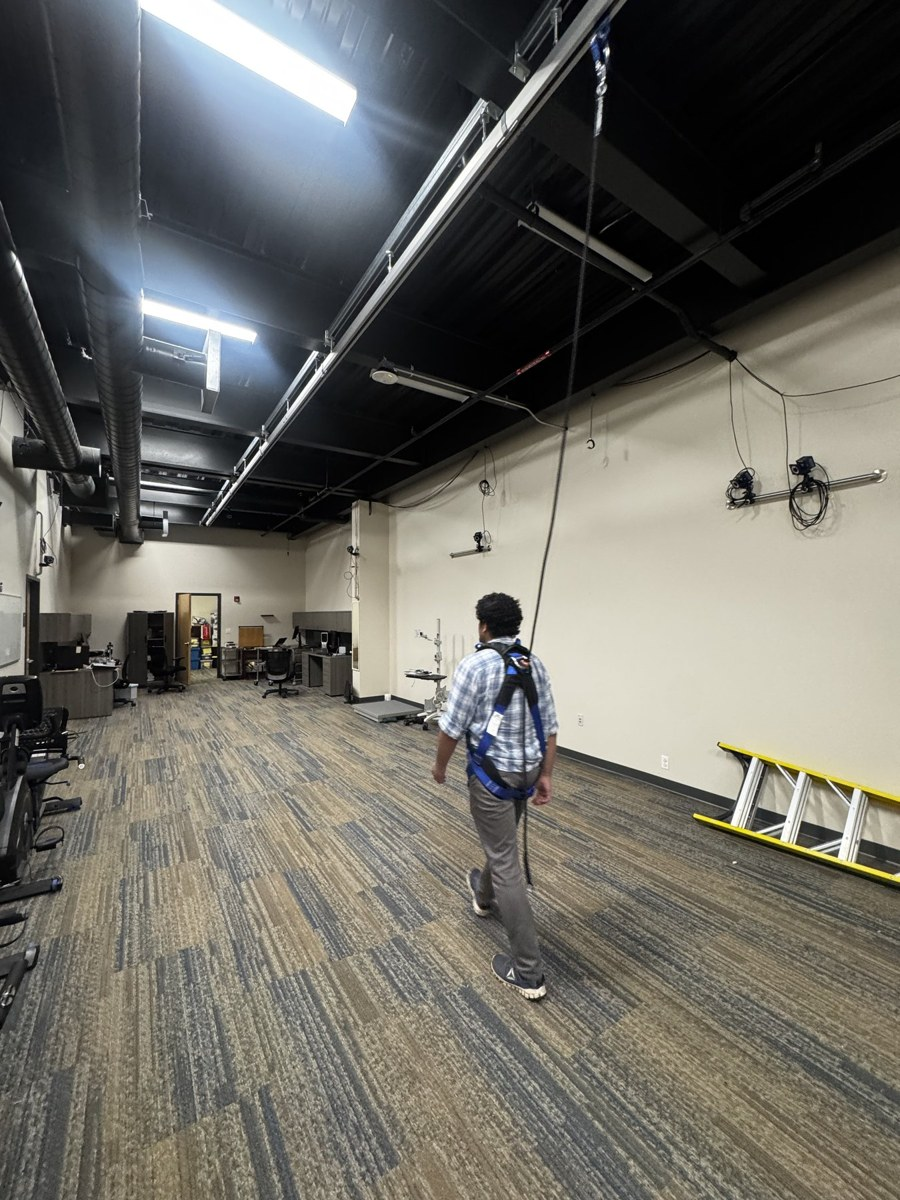
\includegraphics[width=\linewidth]{images/biomech_1.jpg}
\end{minipage}\hfill
\begin{minipage}[t]{0.20\textwidth}
  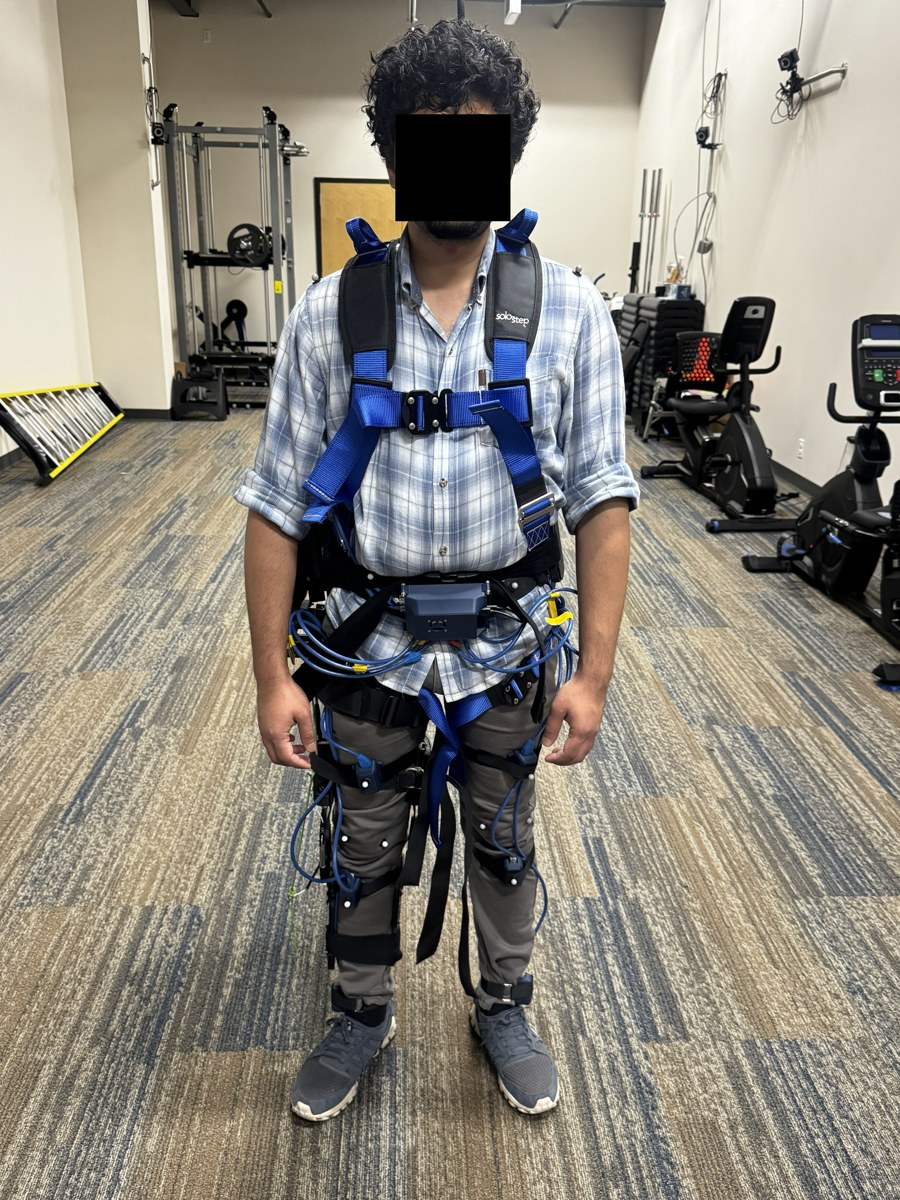
\includegraphics[width=\linewidth]{images/biomech_2.jpg}
\end{minipage}\hfill
\begin{minipage}[t]{0.20\textwidth}
  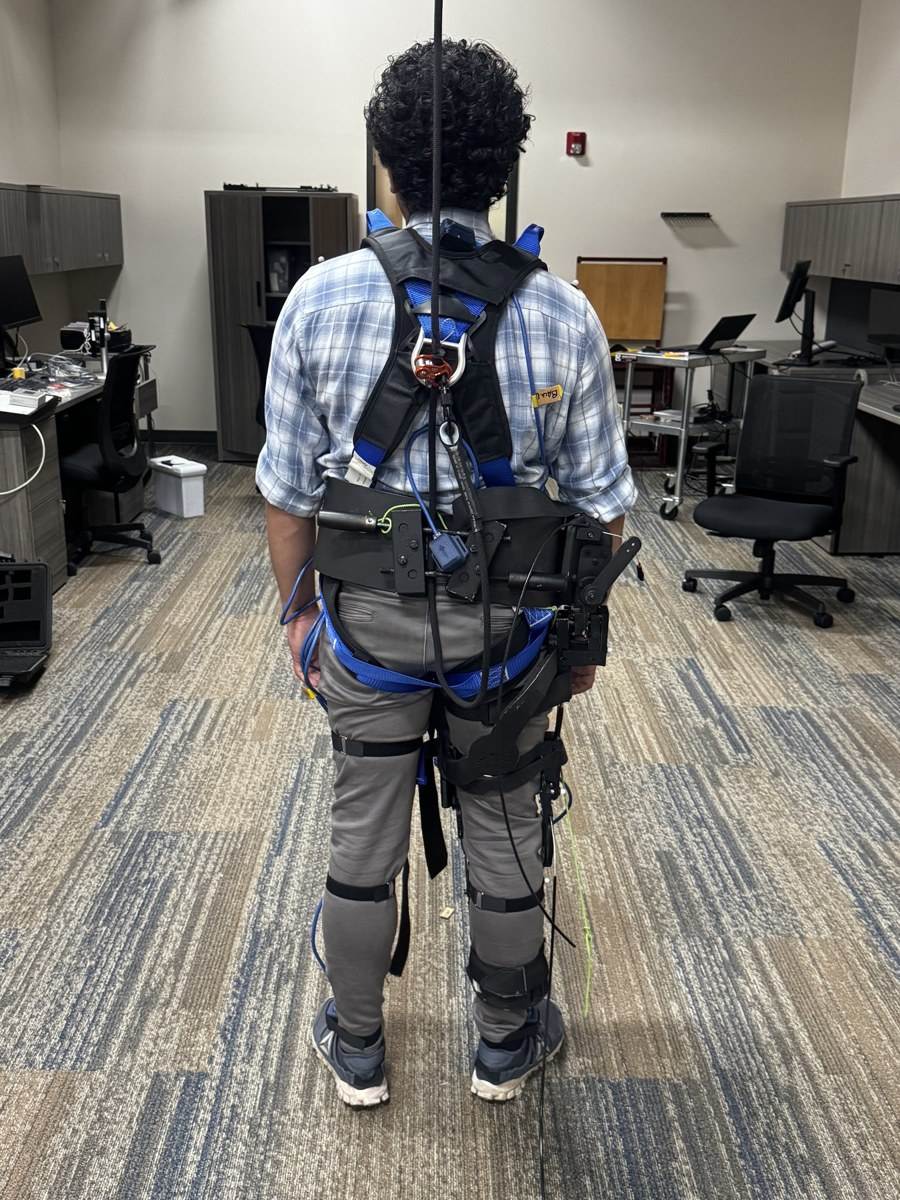
\includegraphics[width=\linewidth]{images/biomech_3.jpg}
\end{minipage}\hfill
\begin{minipage}[t]{0.20\textwidth}
  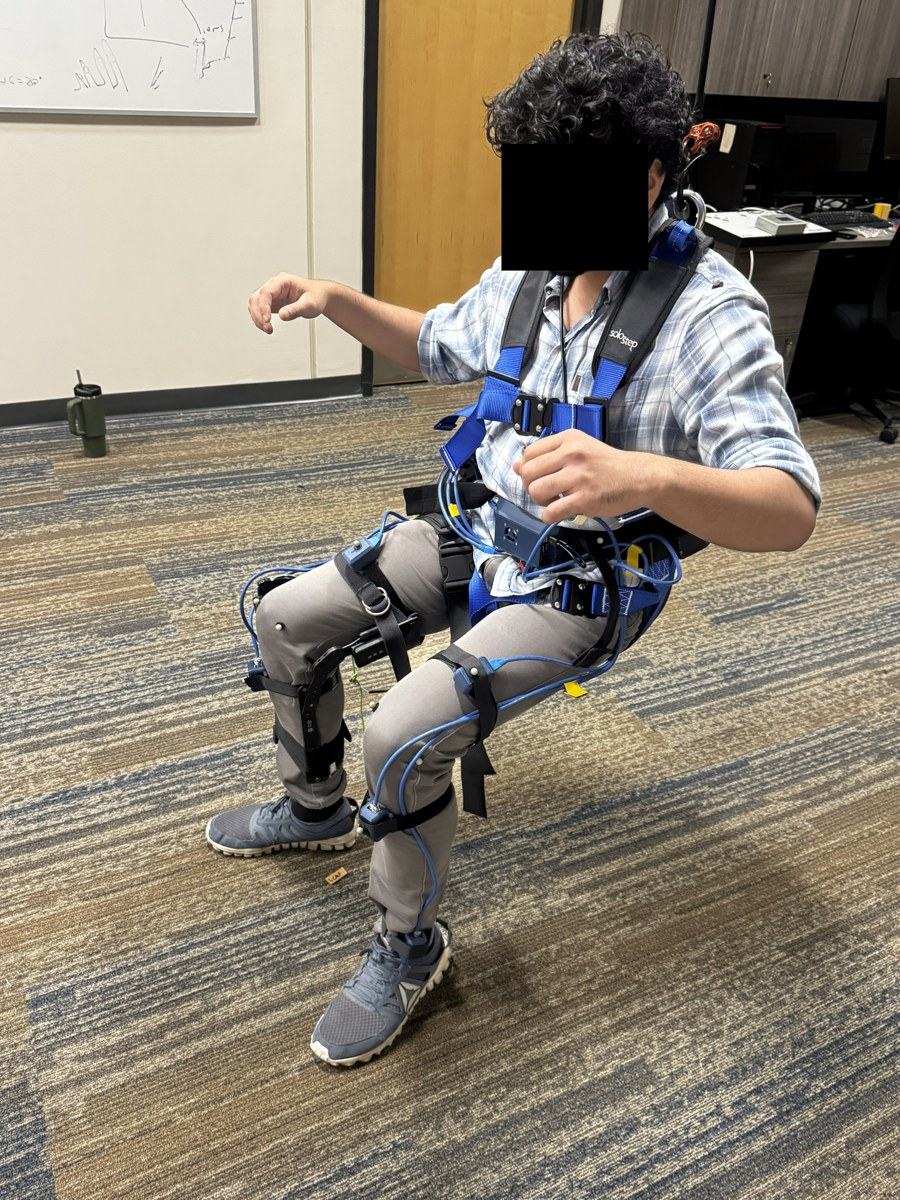
\includegraphics[width=\linewidth]{images/biomech_4.jpg}
\end{minipage}
\captiontext{Worn biomechanics testing on the overhead safety tether:
front, back, and side walking views, and a simulated-fall trial.}

\vspace{4pt}
\begin{minipage}[t]{0.58\textwidth}
In parallel, I am developing an all-in-one backpack that encompasses the
complete control system in a single wearable unit:
\begin{itemize}
  \item Completely new custom electronics, designed to be as compact as
        possible: a custom relay board of my design and custom Control
        Board V2, nearly one-third the size of the previous generation.
  \item Latest edition of the cylinder mechanism, using string-driven
        potentiometers for closed-loop control.
  \item Laser-cut paneling; battery powered, with battery management and
        monitoring.
  \item Pneumatics pressurized via replaceable CO\textsubscript{2}
        canisters for instantaneous release during human trials.
\end{itemize}
Human trials are projected for this fall semester, with a goal of 20
subjects for testing.
\end{minipage}\hfill
\begin{minipage}[t]{0.375\textwidth}
  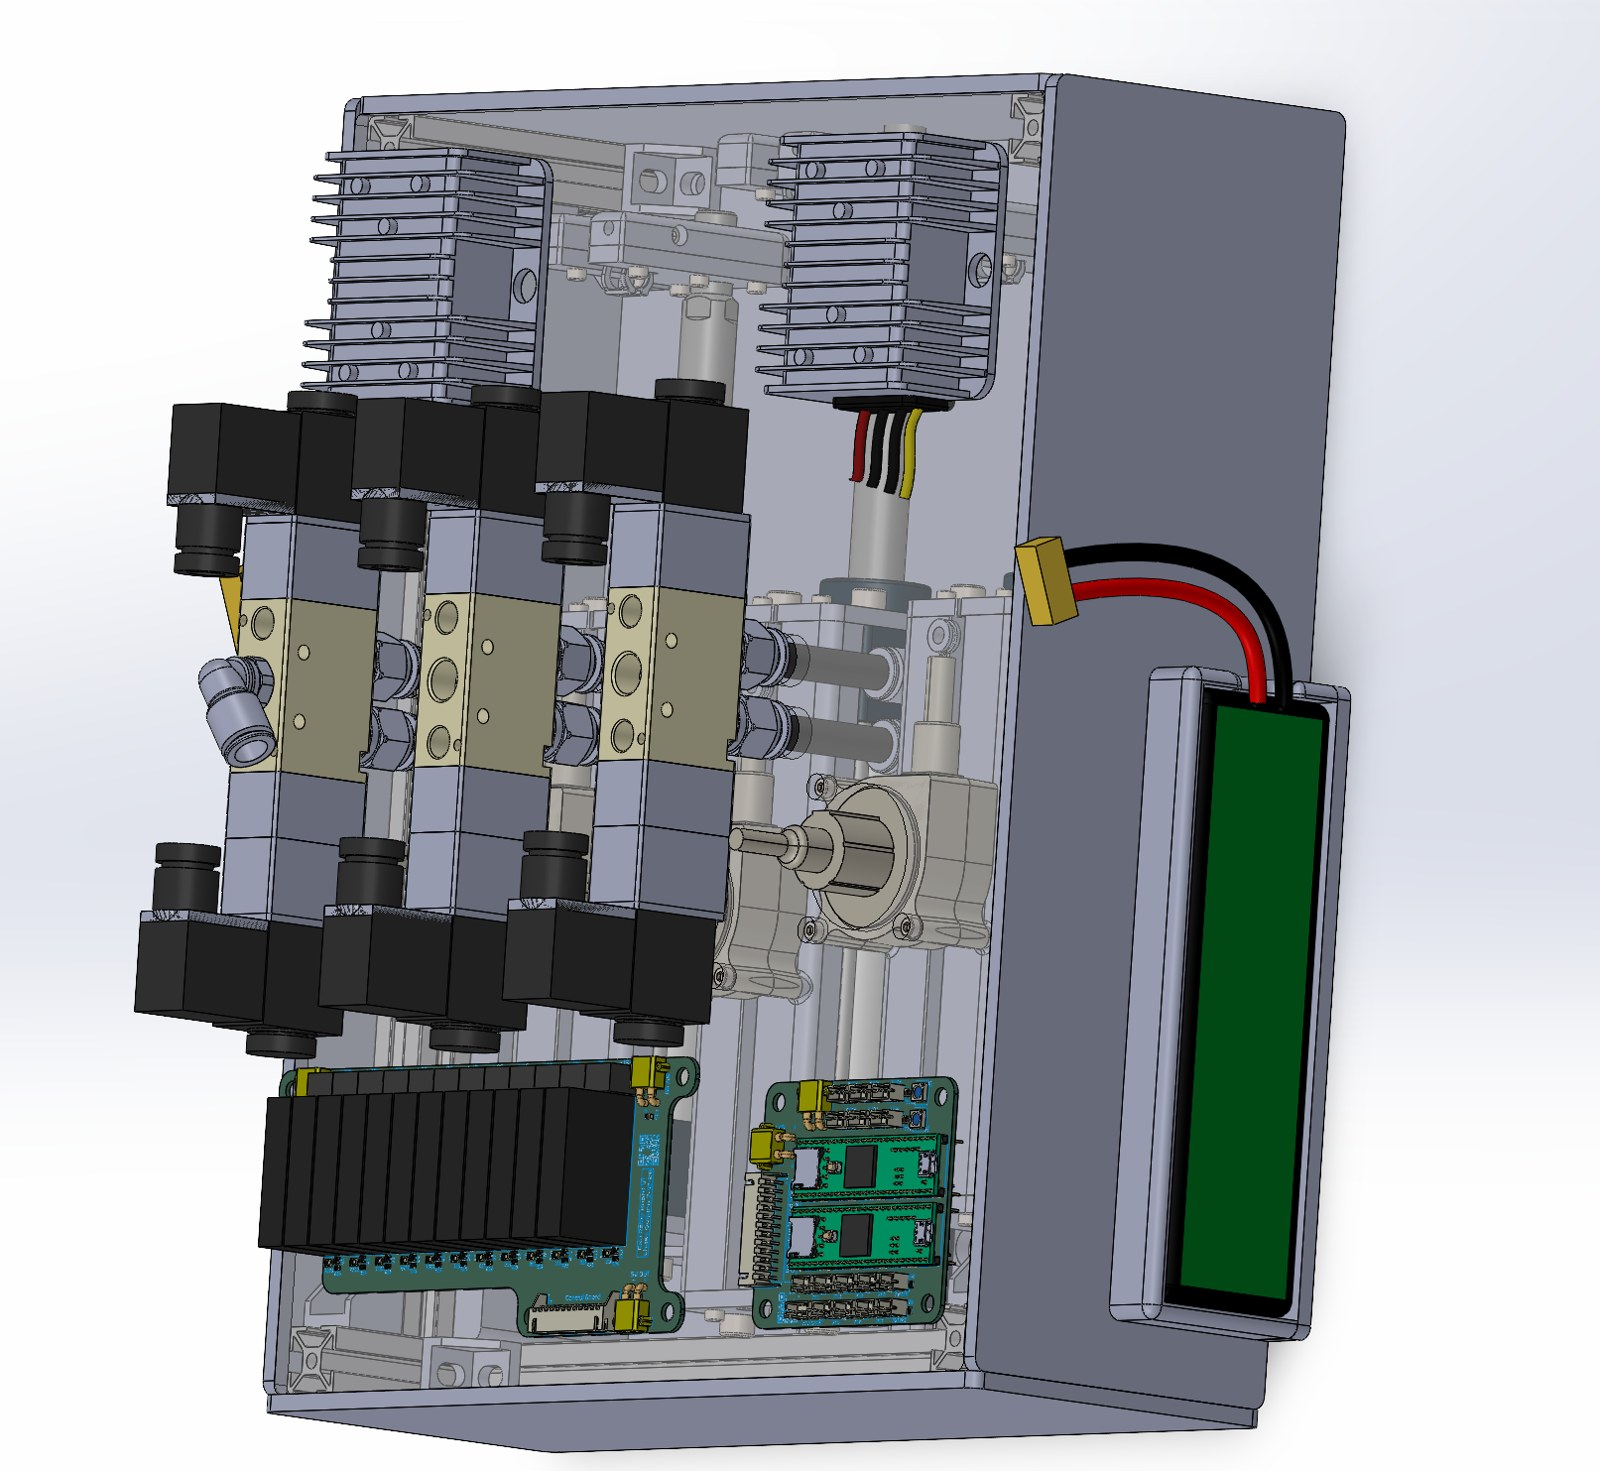
\includegraphics[width=\linewidth]{images/backpack_cad.jpg}
  \captiontext{CAD model progress on the exoskeleton backpack design:
  solenoids, custom relay and control boards, battery, and laser-cut
  paneling in one enclosure.}
\end{minipage}

\vspace{4pt}
\begin{minipage}[t]{0.50\textwidth}
  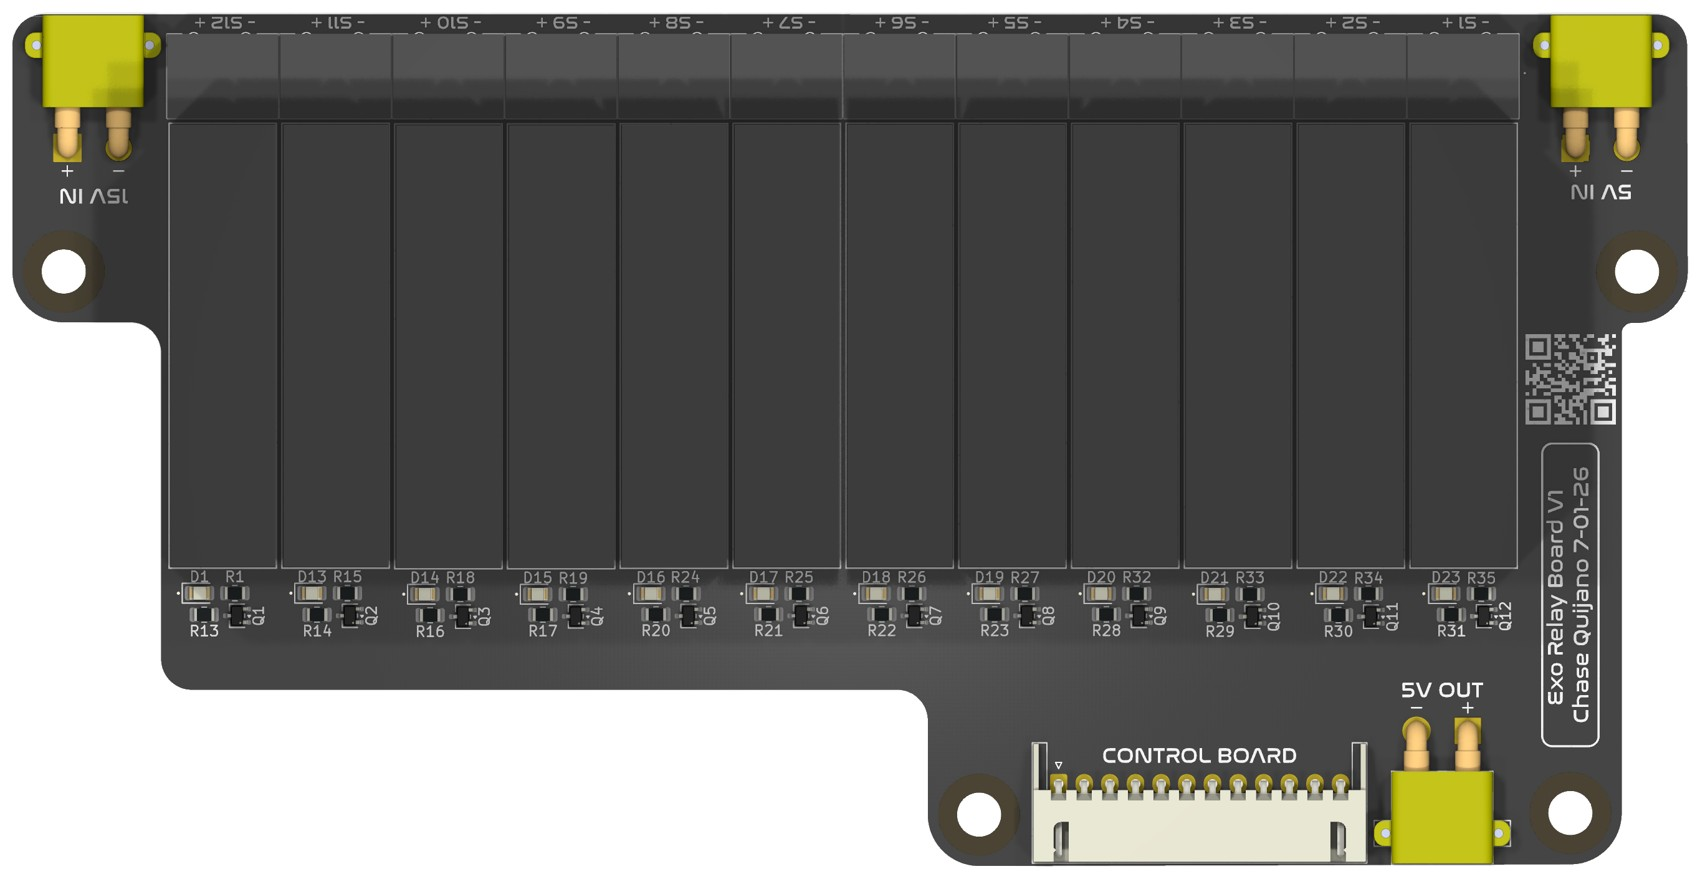
\includegraphics[width=\linewidth]{images/relay_v1_render.jpg}
  \captiontext{Relay Board V1 render: 12-channel, flyback-protected
  relay board of my design for the backpack control system, with switched
  15\,V/5\,V distribution and a dedicated control-board header.}
\end{minipage}\hfill
\begin{minipage}[t]{0.22\textwidth}
  
\includegraphics[width=\linewidth]{images/control_v2_render.jpg}
  \captiontext{Control Board V2 render: primary and secondary
  microcontrollers, with temperature monitoring across multiple systems
  plus pressure and voltage monitoring serving as a safety function, and
  LED status indication.}
\end{minipage}

PhD student Vaibhavsingh Varma and I are preparing for the human trials
and collecting the feedback that will shape the final procedure. I have
been present for all testing throughout my time on the project, will
help run the human trials this fall in the Rowan University biomechanics
lab, and will be a co-author on an upcoming publication from this work.

%== SECTION END =======================================================

\end{document}
